% Options for packages loaded elsewhere
\PassOptionsToPackage{unicode}{hyperref}
\PassOptionsToPackage{hyphens}{url}
%
\documentclass[
]{article}
\usepackage{amsmath,amssymb}
\usepackage{lmodern}
\usepackage{iftex}
\ifPDFTeX
  \usepackage[T1]{fontenc}
  \usepackage[utf8]{inputenc}
  \usepackage{textcomp} % provide euro and other symbols
\else % if luatex or xetex
  \usepackage{unicode-math}
  \defaultfontfeatures{Scale=MatchLowercase}
  \defaultfontfeatures[\rmfamily]{Ligatures=TeX,Scale=1}
\fi
% Use upquote if available, for straight quotes in verbatim environments
\IfFileExists{upquote.sty}{\usepackage{upquote}}{}
\IfFileExists{microtype.sty}{% use microtype if available
  \usepackage[]{microtype}
  \UseMicrotypeSet[protrusion]{basicmath} % disable protrusion for tt fonts
}{}
\makeatletter
\@ifundefined{KOMAClassName}{% if non-KOMA class
  \IfFileExists{parskip.sty}{%
    \usepackage{parskip}
  }{% else
    \setlength{\parindent}{0pt}
    \setlength{\parskip}{6pt plus 2pt minus 1pt}}
}{% if KOMA class
  \KOMAoptions{parskip=half}}
\makeatother
\usepackage{xcolor}
\IfFileExists{xurl.sty}{\usepackage{xurl}}{} % add URL line breaks if available
\IfFileExists{bookmark.sty}{\usepackage{bookmark}}{\usepackage{hyperref}}
\hypersetup{
  pdftitle={Regresjon - Teori},
  hidelinks,
  pdfcreator={LaTeX via pandoc}}
\urlstyle{same} % disable monospaced font for URLs
\usepackage[margin=1in]{geometry}
\usepackage{graphicx}
\makeatletter
\def\maxwidth{\ifdim\Gin@nat@width>\linewidth\linewidth\else\Gin@nat@width\fi}
\def\maxheight{\ifdim\Gin@nat@height>\textheight\textheight\else\Gin@nat@height\fi}
\makeatother
% Scale images if necessary, so that they will not overflow the page
% margins by default, and it is still possible to overwrite the defaults
% using explicit options in \includegraphics[width, height, ...]{}
\setkeys{Gin}{width=\maxwidth,height=\maxheight,keepaspectratio}
% Set default figure placement to htbp
\makeatletter
\def\fps@figure{htbp}
\makeatother
\setlength{\emergencystretch}{3em} % prevent overfull lines
\providecommand{\tightlist}{%
  \setlength{\itemsep}{0pt}\setlength{\parskip}{0pt}}
\setcounter{secnumdepth}{-\maxdimen} % remove section numbering
\newlength{\cslhangindent}
\setlength{\cslhangindent}{1.5em}
\newlength{\csllabelwidth}
\setlength{\csllabelwidth}{3em}
\newlength{\cslentryspacingunit} % times entry-spacing
\setlength{\cslentryspacingunit}{\parskip}
\newenvironment{CSLReferences}[2] % #1 hanging-ident, #2 entry spacing
 {% don't indent paragraphs
  \setlength{\parindent}{0pt}
  % turn on hanging indent if param 1 is 1
  \ifodd #1
  \let\oldpar\par
  \def\par{\hangindent=\cslhangindent\oldpar}
  \fi
  % set entry spacing
  \setlength{\parskip}{#2\cslentryspacingunit}
 }%
 {}
\usepackage{calc}
\newcommand{\CSLBlock}[1]{#1\hfill\break}
\newcommand{\CSLLeftMargin}[1]{\parbox[t]{\csllabelwidth}{#1}}
\newcommand{\CSLRightInline}[1]{\parbox[t]{\linewidth - \csllabelwidth}{#1}\break}
\newcommand{\CSLIndent}[1]{\hspace{\cslhangindent}#1}
\usepackage{booktabs}
\usepackage{longtable}
\usepackage{array}
\usepackage{multirow}
\usepackage{wrapfig}
\usepackage{float}
\usepackage{colortbl}
\usepackage{pdflscape}
\usepackage{tabu}
\usepackage{threeparttable}
\usepackage{threeparttablex}
\usepackage[normalem]{ulem}
\usepackage{makecell}
\usepackage{xcolor}
\usepackage{multicol}
\usepackage{hhline}
\usepackage{hyperref}
\ifLuaTeX
  \usepackage{selnolig}  % disable illegal ligatures
\fi

\title{Regresjon - Teori}
\author{}
\date{\vspace{-2.5em}}

\begin{document}
\maketitle

\hypertarget{innledning}{%
\section{Innledning}\label{innledning}}

Regresjonsanalyse er et særtilfelle av variansanalyse, og er i følge
Mehmetoglu and Mittner (2020) muligens en mest brukte analysemetoden for
dataanalyse, eller arbeidshesten i foskning på økonomiske og sosiale
forhold (Thrane 2019). Det er først og fremst metodens er fleksibilitet
som en hovedgrunn til dette.

En regresjonsanalyse er en en statistisk analyse som undersøker
sammenhengen mellom en kontinuerlig avhengig variabel og en eller flere
kontinuerlige og/eller kategoriske uavhengige variabler
@{[}mehmetogluInnforingStatistiskeDataanalyser2020{]}. Selv om
korrelasjon kan være veldig hjelpsomt å forstå vil en regresjonsanalyse
søke å ta vår forståelse av sammenhengen litt videre, til for eksempel å
forsøke å predikere nivået i en avhengig variabel ut fra nivået på
den/de uavhengige variabler. Hvis vi lykkes med dette vil vi kunne klare
å si noe om forventet verdi på et fenomen vi er interessert i ut fra
kjente verdier på andre variabler. La oss anta at vi har variabler som
beliggenhet (avstand fra sentrum), areal, etasje, solforhold, antall
rom, antall bad, standard på bad og liknende for en leilighet kan vi
bruke disse uavhengige variablene til å predikere en salgssum for denne
boligen (som en avhengig variabel). Vi lager da en modell for dette
forholdet - i dette tilfellet en regresjonsmodell. Vi går dermed fra å
spørre \textbf{om} det er en sammenheng til å spørre \textbf{hvilken}
sammenheng det er.

Denne innledningen til regresjonsanalyse tar utgangspunkt i eksempelet i
Løvås (2013) (boka kom ut i 4. utgave i 2018). Illustrasjonene som er
brukt er hentet fra bokas
\href{www.nettressurser.no/statistikk}{nettressurser}. Løvås' bok
«Statistikk for universiteter og høgskoler» kan anbefales som
introduksjonsbok til statistikk på universitets- og høgskolenivået. En
annen bok som fungerer fint til dette formålet er Jan Ubøes ``Statistikk
for økonomifag'' (vi har brukt 4. utgave, 2014 - 5. utgave kom i 2015)
(Ubøe 2014).

\hypertarget{teori}{%
\section{Teori}\label{teori}}

Eksempelet i Løvås (2013) dreier seg om sammenhengen mellom
motorstørrelse og drivstofforbruk. Vi kan måle motorstørrelse i
hestekrefter (hk) og drivstofforbruk i liter/mil.

For å vise sammenhengen kan vi sette opp ligningen
\(Y_i=\alpha\:+\beta x_i+e_i\) der

\(Y=drivstofforbruket\)

\(\alpha=konstantleddet\) (krysningspunktet på y-aksen, altså Y-ver dien
om x er 0)

\(\beta=linjens\:stigningstall\) (dersom x øker med 1, øker y med
\(\beta\)

\(e=forstyrrelsen\) (vi antar at det er flere ting som forstyrrer
forholdet mellom motorstørrelse og drivstofforbruk - drivstofforbruket
er ikke bare avhengig av motorstørrelse). Vi skal snakke mye om
residualer i regresjonsanalyse - residualer er dette
restleddet/feilleddet/forstyrrelsen. En av forutsetningene i
regresjonsanalyse er knyttet til fordelingen av disse residualene, men
det kommer vi tilbake til.

Dersom vi ikke hadde hatt et feilledd kunne vi framstilt denne ligningen
slik:

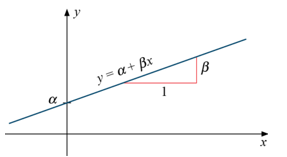
\includegraphics{Teori_fig1.png}

Når vi plotter inn et antall observasjoner av motorstørrelse og
drivstofforbruk kan det se slik ut:

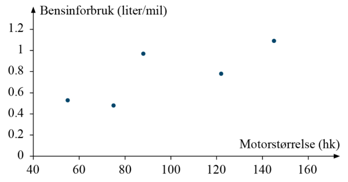
\includegraphics{Teori_fig2.png}

Det vi i en lineær regresjonsanalyse gjør er å finne den rette linja som
best passer til disse observasjonene. Vi ønsker altså å finne en rett
linje som best «beskriver» observasjonene. Tenk deg at vi trekker den
rette linja som samlet sett ligger nærmest punktene og deretter tar bort
punktene. Det vi sitter igjen med er regresjonslinja. Denne linja gir
oss da ``tilgang til'' alle punkter som ligger på linja som en modell på
sammenhengen mellom de to variablene. Selv om vi bare hadde noen
observasjoner på gitte punkter på x-aksen har vi gjennom regresjonslinja
fått tilgang til alle tenkelige punkter på x-linja og kan anta et
drivstofforbruk ut fra det (ved å gå opp fra x-aksen, finne
skjæringspunktet med regresjonslinja, og deretter gå inn på y-aksen og
lese av drivstofforbruket). Den prediksjonen vi da gjør er vår beste
gjetning på hvor stort drivstofforbruket vil være for en gitt
motorstørrelse. Dette vil selvsagt være en kvalifisert gjetning -
nettopp fordi det er en modell. Og alle modeller er feil, men noen
modeller er nyttige likevel.

I eksempelet kan vi for eksempel tenke oss to mulige linjer:

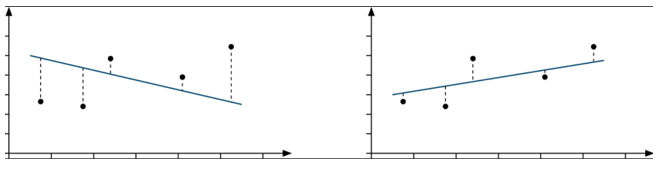
\includegraphics{Teori_fig3.png}

Begge linjene er forsøk på å lage en rett linje som har kortest mulig
avvik. Vi kan deretter legge sammen de absolutte vertikale avstandene
(de stiplede linjene) fra observasjonspunktene ned til den rette linja.
I prinsippet er da den rette linja som medfører minst samlet avstand fra
observasjonspunktene den rette linja som best representerer
observasjonspunktene, og vi kan si vi har laget en modell for
sammenhengen mellom motorstørrelse og drivstofforbruk. Siden vi har en
sammenhengende rett linje har vi også mulighet til å mene noe om
drivstofforbruk på motorstørrelser vi ikke har målt/har observasjoner
på. Vi har med andre ord en modell for å predikere drivstofforbruk ut
fra motorstørrelse. Uavhengige variabler i regresjonsanalyser kalles
også ofte prediktorer, fordi vi bruker de til å predikere en verdi for
den avhengige variabelen.

\hypertarget{minste-kvadratsum-ordinary-least-squares---ols}{%
\subsection{Minste kvadratsum (Ordinary Least Squares -
OLS)}\label{minste-kvadratsum-ordinary-least-squares---ols}}

Imidlertid er absoluttverdier matematisk problematiske (Løvås 2013).
Pre-datamaskiner ble det derfor utviklet en alternativ måte som kalles
«minste kvadraters metode» - derav begrepet OLS («Ordinary Least
Squares»). Det finnes andre måter å tilnærme seg dette, men i dette
kurset går vi kun inn på OLS-regresjon.Hvis vi fortsetter eksempelet
over kan vi tenke oss en mengde forslag på ulike linjer som forsøker å
beskrive sammenhengen mellom de to variablene:

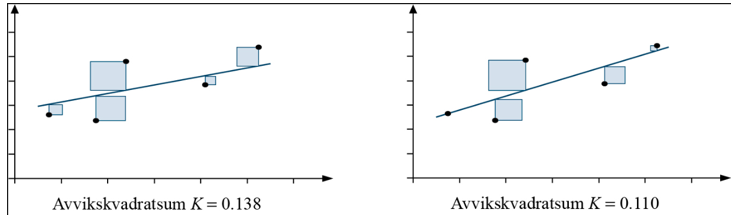
\includegraphics{Teori_fig4.png}

Man regner deretter ut kvadratene som dannes av hvert punkt og avstanden
til den rette linja. Den linja som har den laveste kvadratsummen («least
squares») er den linja som best representerer datapunktene og som derfor
er den beste lineære modellen av forholdet mellom variablene.
Regresjonslinja er således en modell. Som Thrane (2019) beskriver: den
diagonale linja oppsummerer den typiske trenden i det statistiske
forholdet mellom de to variablene - en linje vi kjenner som
regresjonslinja. Hvis vi har et stort antall datapunkter er dette
selvsagt en omfattende prosess å gjøre manuelt. Det program som jamovi
gjør for oss er å regne ut kvadratsummen for et stort antall mulige
linjer og deretter fortelle oss hvilken som har lavest kvadratsum.

Hvis vi tenker tilbake til formelen for modellen vår:
\(Y_i=\alpha\:+\beta x_i+e_i\) kan vi nå fylle ut med verdier fra
eksempelet.

Det vi egentlig har gjort når vi finner den rette linja som gir minste
kvadratsum er å identifisere \(\alpha\) (skjæringspunktet på y-aksen) og
\(\beta\) (stigningstallet). Jamovi vil gi oss verdiene på dette. Vi går
ikke inn på en manuell utregning her, men bruker de to verdiene Løvås
(2013) viser (\(\alpha=0.211\) og \(\beta=0.00576\)). Vår modell ser da
slik ut: \(Y_i=0,211\:+0,00576x_i\).

Som sagt har vi ønsket å lage en modell som predikerer drivstofforbruk
ut fra motorstørrelse -- eller sagt på en annen måte: hvilket
drivstofforbruk kan vi forvente med en motor på 100 hk? Vi får da:
\[Y_i=0,211\:+0,00576x_i=0,211\:+\:0,00576\times100\:=\:0,787\]

Dette blir vårt ``best guess'', vår antakelse (vår prediksjon av verdien
på y-aksen som er drivstofforbruket ut fra verdien på x-aksen som er
motorstørrelse), om forventet drivstofforbruk for en motor med 100 hk
basert på den modellen vi har laget om sammenhengen mellom
motorstørrelse og drivstofforbruk (som er basert på de observasjonene vi
har).

Vi kan naturligvis umiddelbart tenke at drivstofforbruket er avhengig av
mange andre faktorer enn motorstørrelse, for eksempel bilens design
(luftmotstand), vekt, rullemotstand, temperatur, type motor og så
videre. Dette belyser for så vidt et sentralt problem når vi ønsker å
lage modeller for prediksjon: Virkeligheten er utrolig sammensatt, mange
relevante variabler er vanskelig å måle, og man ønsker en modell som er
enkel nok til å kunne brukes og sammensatt nok til å gi relevante
prediksjoner. Tenk for eksempel bare på «klimamodellene» som brukes for
å analysere og predikere temperatur, issmelting, global oppvarming og
liknende. Det er klart at i de fleste tilfeller trenger vi flere
prediktorer enn en -- og i regresjonssammenheng snakker vi da om
multippel regresjonsanalyse. Vi kan ha som en tommelfingerregel at vi
skal ha med så mange variabler at modellen har praktisk verdi, men
likevel så få som mulig.

\hypertarget{konfidensintervall}{%
\section{Konfidensintervall}\label{konfidensintervall}}

Avslutningsvis i denne introduksjonen til regresjonsanalyse kan vi se
kort på begrepet konfidensintervall (se for eksempel Løvås (2013) eller
Hinkle, Wiersma, and Jurs (2003)).For de som ønsker å fordype seg i
effektstørrelser og konfidensintervaller anbefales Cumming and
Calin-Jageman (2017) ``Introduction to the new statistics: Estimation,
open science, \& beyond''.

Man kan si at estimatet på stigningstallet \(\beta\) er det viktigste
resultatet i en regresjonsanalyse fordi dette sier noe om hvor sterk
sammenhengen mellom de to variablene er. Løvås (2013) illustrerer dette
slik:

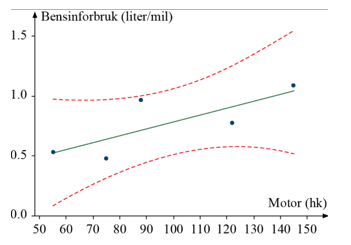
\includegraphics{Teori_fig5.png}

De røde stiplede linjene utgjør konfidensgrensene for 95 \%
konfidensintervall. I grafen over har vi kun 5 observasjoner, noe som
selvsagt er lite. Vi kan gå litt dypere inn i hvordan konfidensgrensene
framkommer i en regresjonsanalyse.

La oss anta at vi har et datasett der vi har plottet korrelasjonen
mellom en prediktor (den uavhengige variabelen) på x-aksen og en
avhengig varaibel på y-aksen (se graf under). Den røde prikken markerer
verdien x=8. Verdien på y-aksen (10,458) er vår prediksjon (vår buest
guess) på hva verdien i den avhengige variabelen vil være ved den
observerte verdien x=8.

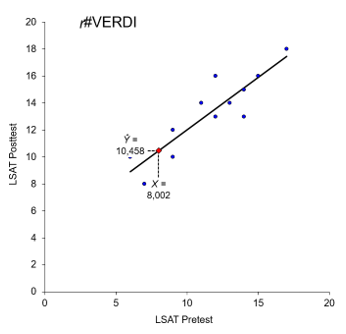
\includegraphics{Teori_fig6.png}

I punktet x=8 har vi en hel populasjon av mulige normalfordelte verdier.
Vårt beste estimat av gjennomsnittsverdien for denne populasjonen er
10,458. Dette er et punktestimat. Det tilhørende intervallestimatet er
vårt konfidensintervall. Vi må her tenke på konfidensintervallet som en
vertikal linje. Så i stedet for å tenke punkt- og intervallestimat slik

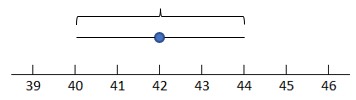
\includegraphics{Teori_fig7.png}

Kan vi tenke det slik:

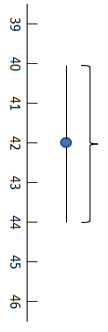
\includegraphics{Teori_fig8.png}

Overført til vårt eksempel får vi:

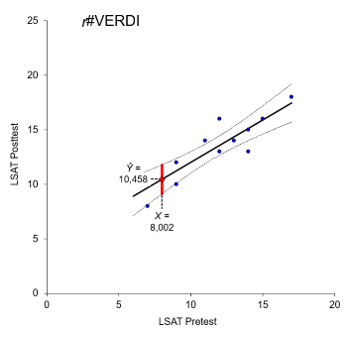
\includegraphics{Teori_fig9.png}

Den røde streken er vårt 95 \% konfidensintervall for punktestimatet.
Hvis vi legger på 95 \% konfidensintervaller på alle punktestimatene
(alle punktene som utgjør regresjonslinja) kan vi lage de to stiplede
linjene som toucher endepunktene på alle konfidensintervallene. Disse to
stiplede linjene utgjør da konfidensgrensene for regresjonslinja.

Vi ser at konfidensgrensene er lett buede mot hverandre med minst
avstand mellom dem ``på midten''. Vi skal kort se på hvorfor det er
slik. Vi har nå lagt på et nytt kryss i grafen under. Dette krysset
markerer punktet der gjennomsnittene av X og Y krysser. Regresjonslinja
må gå gjennom dette punktet, slik at alle alternative regresjonslinjer
må pivotere rundt dette punktet. Dette medfører at det er litt større
usikkerhet rundt punktestimatenes konfidensintervaller i endene i
forhold til i midten. Konfidensintervallene for hvert enkelt punkt blir
derfor litt lenger jo lenger ut fra krysningspunket vi går, og
resultatet blir en form for buet linje.

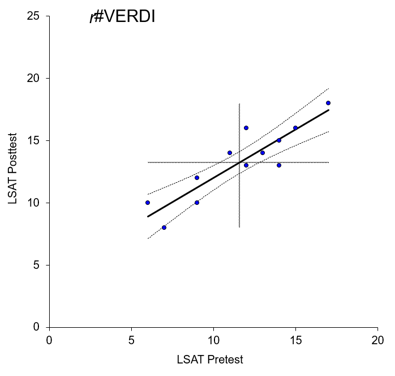
\includegraphics{Teori_fig10.png}

\hypertarget{steg-i-analyse}{%
\section{Steg i analyse}\label{steg-i-analyse}}

Vi anbefaler at en analyse går gjennom disse stegene:

\begin{enumerate}
\def\labelenumi{\arabic{enumi}.}
\item
  Analyse av dataene
\item
  Evtentuelt valg av prediktorer ut fra analyse av dataene
\item
  Lage modell (kjøre regresjonsanalysen)
\item
  Analyse av resultatene (diagnostikk)
\item
  Sjekk av forutsetningene
\item
  Eventuell revisjon av modellen
\item
  Eventuell analyse av revidert modell
\item
  Konklusjon / oppsummering / rapportering av resultater
\end{enumerate}

Vi skal i det følgende gå gjennom disse stegene i en regresjonsanalyse.

\hypertarget{enkel-lineuxe6r-regresjonsanalyse}{%
\section{Enkel, lineær
regresjonsanalyse}\label{enkel-lineuxe6r-regresjonsanalyse}}

Dette eksempelet bygger på Field (2009). Du kan laste ned datasettet i
ulike formater her:

Datasettet kan også finnes
\href{https://edge.sagepub.com/field5e/student-resources/datasets}{her}

Vi skal nå gå gjennom våre anbefalte steg i analysen, og starter med en
analyse av dataene.

\hypertarget{steg-1-analyse-av-dataene}{%
\subsection{Steg 1: Analyse av
dataene}\label{steg-1-analyse-av-dataene}}

Vi ser på datasettet.

\begin{verbatim}
## # A tibble: 200 x 4
##    Adverts Sales Airplay Image
##      <dbl> <dbl>   <dbl> <dbl>
##  1    10.3   330      43    10
##  2   986.    120      28     7
##  3  1446.    360      35     7
##  4  1188.    270      33     7
##  5   575.    220      44     5
##  6   569.    170      19     5
##  7   472.     70      20     1
##  8   537.    210      22     9
##  9   514.    200      21     7
## 10   174.    300      40     7
## # ... with 190 more rows
\end{verbatim}

Vi kan se at datasettet består av 200 obervasjoner av 4 variabler. Hver
av observasjonene er en CD:

\begin{itemize}
\tightlist
\item
  Adverts: Dette er summen brukt på reklame før lanseringsdato
\item
  Sales: Dette er salgtall per uke
\item
  Airplay: Antall ganger et spor fra CDen ble spilt på radio i uka før
  lanseringsdato
\item
  Image: En rating på hvor attraktiv (positivt image) gruppen/artisten
  har
\end{itemize}

Hvis vi ønsker å se på i hvilken grad vi kan predikere salgstall gjennom
hvor mye vi bruker på reklame før lansering kan vi gjøre en lineær
regresjonsanalyse med salg som avhengig variable og reklame (adverts)
som uavhengig variabel.

I en analyse av dataene kan vi for eksempel være interessert i noen
nøkkeltall:

\begin{verbatim}
##     Adverts             Sales          Airplay          Image      
##  Min.   :   9.104   Min.   : 10.0   Min.   : 0.00   Min.   : 1.00  
##  1st Qu.: 215.918   1st Qu.:137.5   1st Qu.:19.75   1st Qu.: 6.00  
##  Median : 531.916   Median :200.0   Median :28.00   Median : 7.00  
##  Mean   : 614.412   Mean   :193.2   Mean   :27.50   Mean   : 6.77  
##  3rd Qu.: 911.226   3rd Qu.:250.0   3rd Qu.:36.00   3rd Qu.: 8.00  
##  Max.   :2271.860   Max.   :360.0   Max.   :63.00   Max.   :10.00
\end{verbatim}

Ofte er det imidlertd mer hensiktsmessig å se på dataene grafisk i en
utforskende hensikt (Tukey 1977).

\hypertarget{histogram}{%
\subsubsection{Histogram}\label{histogram}}

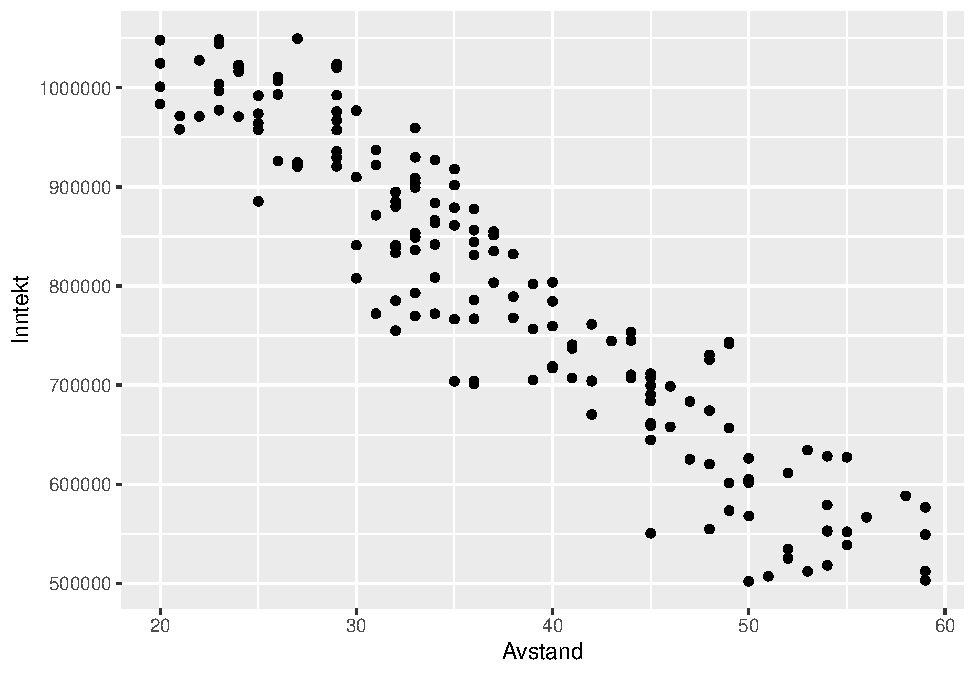
\includegraphics{Regresjon_Teori_files/figure-latex/unnamed-chunk-7-1.pdf}
Det kan se ut som at salgstallene er rimelig normalfordelte, mens
reklamevariabelen er klart skjev.

\hypertarget{quantile-quantile-plott-qq}{%
\subsubsection{Quantile-Quantile plott
(qq)}\label{quantile-quantile-plott-qq}}

Q-Q plottet (``quantile-quantile plot'') kan tolkes ved å se om
dataverdiene ligger langs en rett linje med ca 45 graders vinkel. Q-Q
plottet (se video for forklaring på utregning) innebærer å se to
distribusjoner mot hverandre -- empirisk fordeling (dataene) og
teoretisk forventning ut fra en fordelingsmodell (som normalfordeling om
vi snakker om ``normal Q-Q plott - dvs vi ser om vår empiriske
datafordeling og normalfordelingen er lik). Om de samsvarer perfekt
ligger de på en helt rett linje (x = y). I eksempelet under vil da alle
punktene ligge perfekt oppå den rette linjen. Siden vi vet den
teoretiske distribusjonen til normalfordelingen, kan vi bruke denne
teoretiske fordelingen til å plotte den mot datasettet vi sitter med.
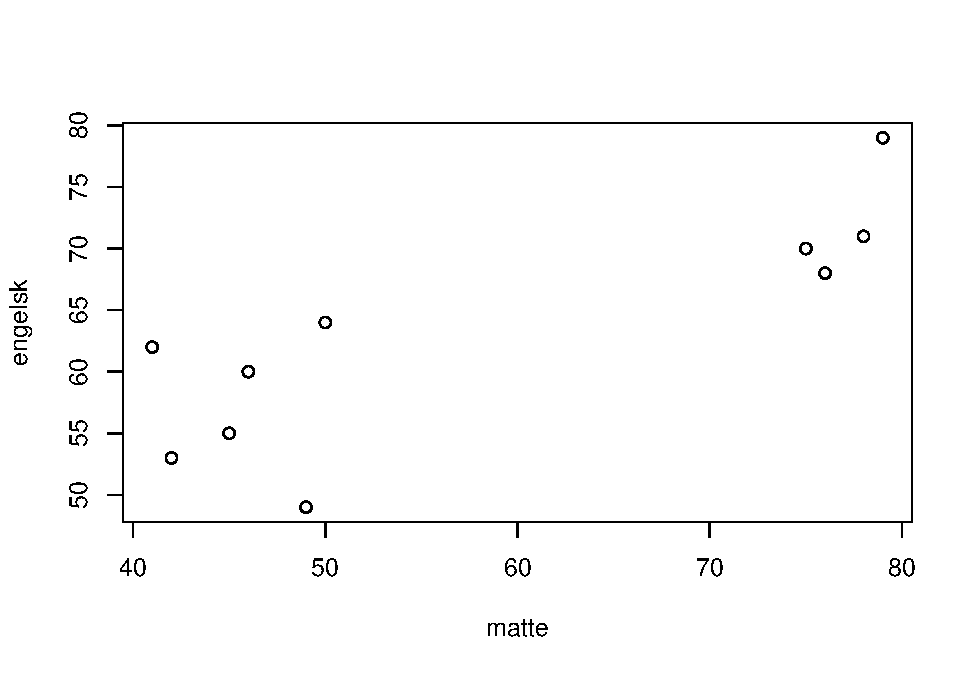
\includegraphics{Regresjon_Teori_files/figure-latex/unnamed-chunk-8-1.pdf}
Som vi fikk indikert gjennom historgrammene er salgsvariabelen rimelig
normalfordelt, mens reklamevariabelen viser avvik fra normalfordelingen
- i dette tilfellet (ut fra histogram og qq-plott vil vi si den er
høyreskjev).

Under viser vi typiske mønstre for histogram og ``tilhørende'' qq-plott
som kan være til hjelp i tolkning av dataene dine. Dette er genererte
tall og ikke tallene fra eksempelet over:

\hypertarget{normalfordelt}{%
\paragraph{Normalfordelt}\label{normalfordelt}}

\begin{figure}
\centering
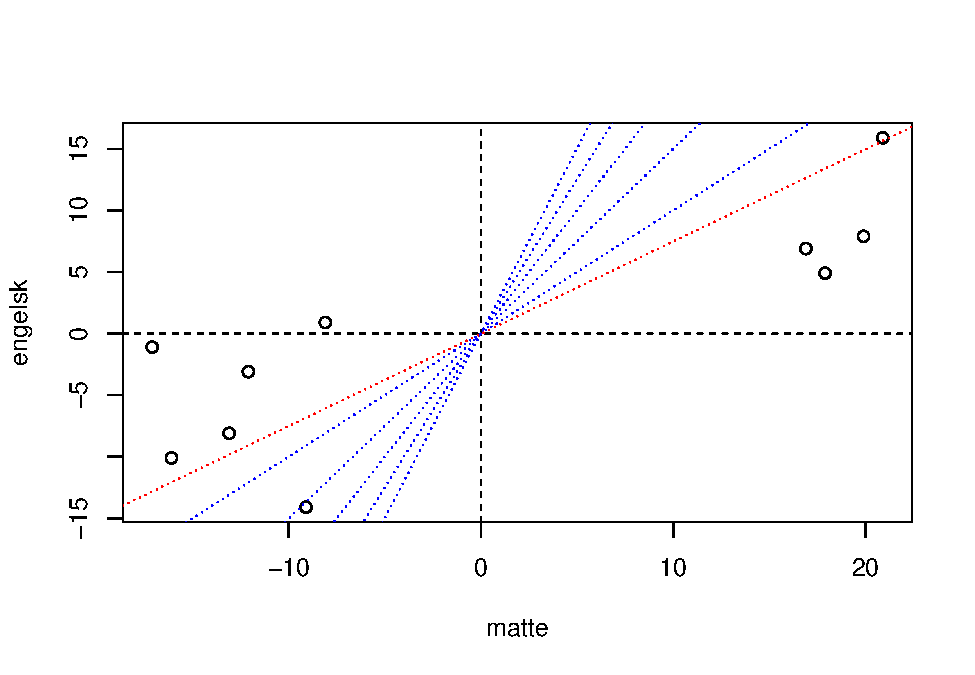
\includegraphics{Regresjon_Teori_files/figure-latex/unnamed-chunk-11-1.pdf}
\caption{Q-Q plott normalfordeling}
\end{figure}

Vi ser at dette Q-Q plottet viser oss at vi kan være ganske sikre på at
dette datasettet er normalfordelt (noe som gir meninig siden vi har
brukt R til å lage et normalfordelt datasett).

\hypertarget{skjevhet-huxf8yre}{%
\paragraph{Skjevhet høyre}\label{skjevhet-huxf8yre}}

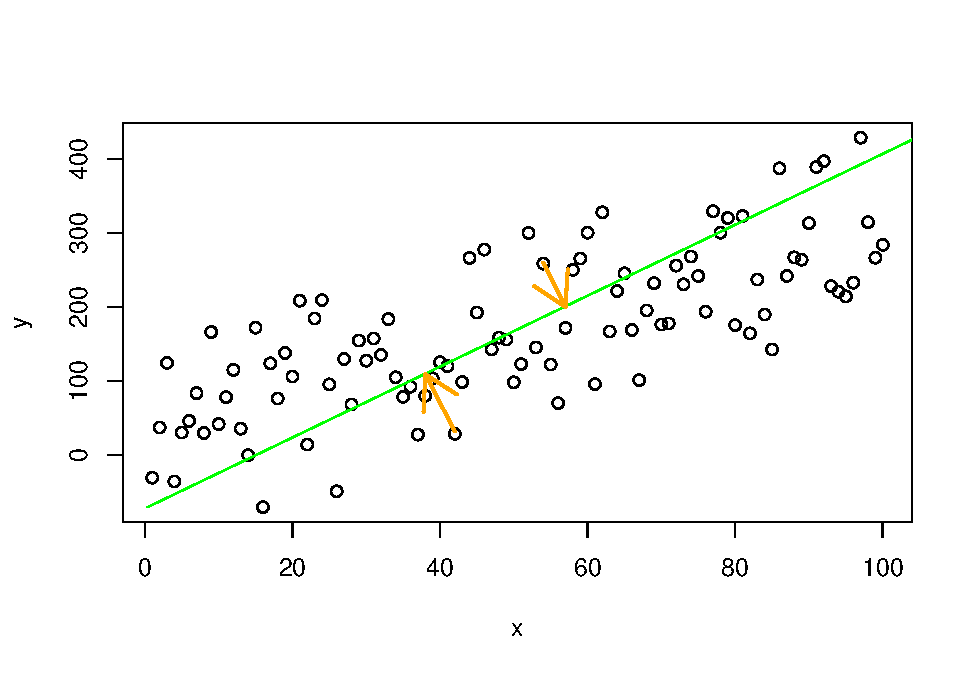
\includegraphics{Regresjon_Teori_files/figure-latex/unnamed-chunk-14-1.pdf}
I et datasett med høyreskjevhet vil ofte Q-Q plottet vise en bananform
med ``bunnen''/midten av bananen ned mot høyre hjørne og endene pekende
oppover/utover fra den rette linjen.

\hypertarget{skjevhet-venstre}{%
\paragraph{Skjevhet venstre}\label{skjevhet-venstre}}

\begin{figure}
\centering
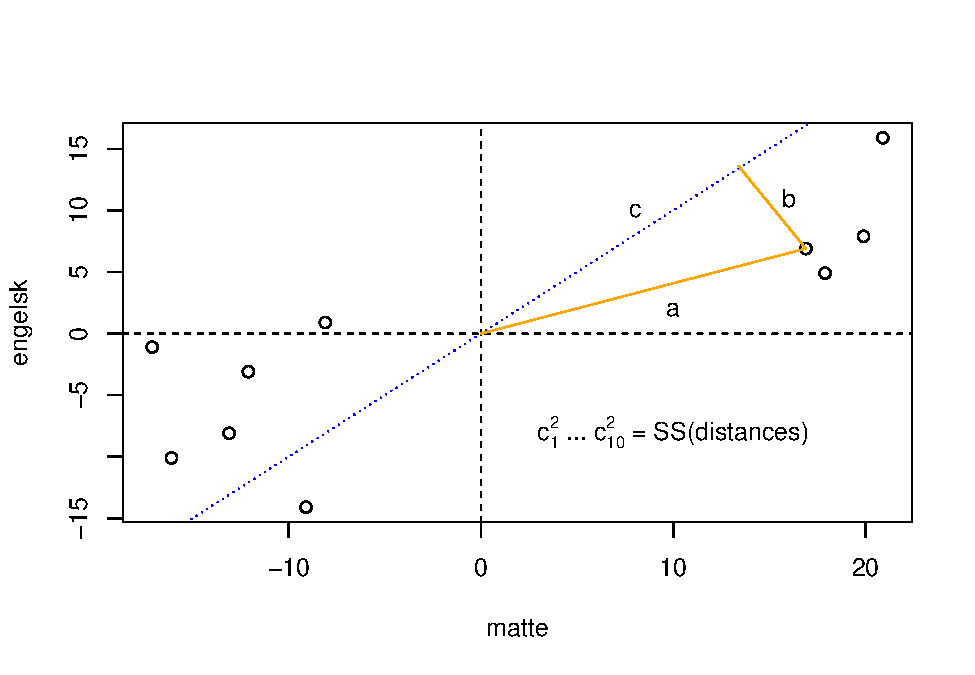
\includegraphics{Regresjon_Teori_files/figure-latex/unnamed-chunk-17-1.pdf}
\caption{Q-Q plott - fordeling skjevhet venstre}
\end{figure}

I dette datasettet har vi generert en kraftig skjevhet til venstre. Q-Q
plottet får da en omvendt bananform i forhold til høyre skjevhet, altså
en topp på midten og to ender som svinger nedover ift den rette linja.

\hypertarget{tunge-haler}{%
\paragraph{Tunge haler}\label{tunge-haler}}

\begin{figure}
\centering
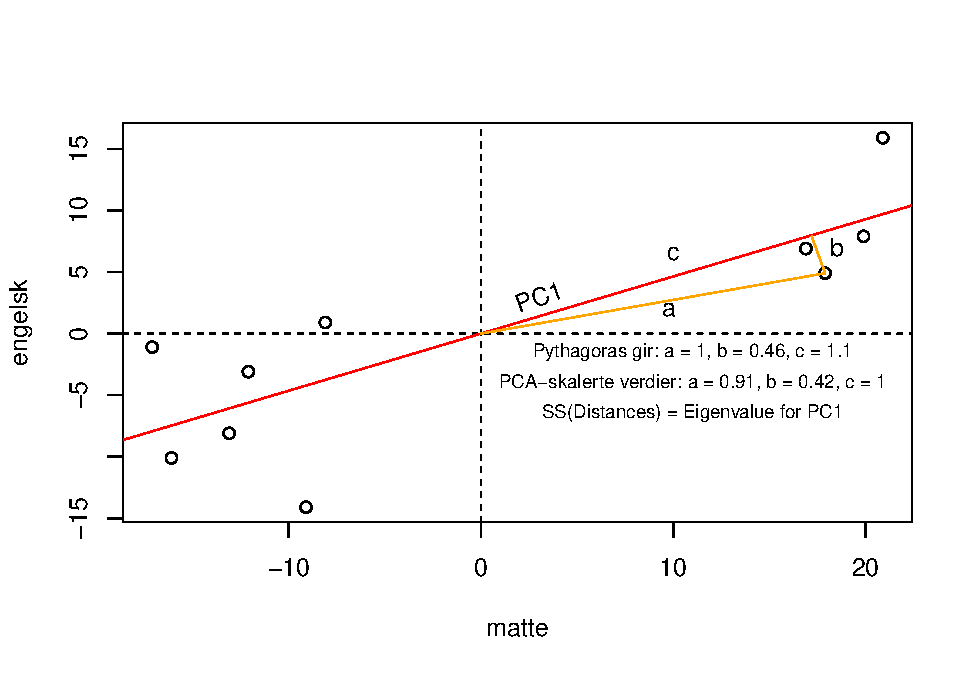
\includegraphics{Regresjon_Teori_files/figure-latex/unnamed-chunk-20-1.pdf}
\caption{Q-Q plott - `heavy-tail'}
\end{figure}

``Heavy-tailed'' (fete/tunge haler) har større sannsynlighet for at
ekstreme verdier vil forekomme). Fordelinger med tunge haler vil ofte
følge en slags S-form, men den er ofte mer ``liggende'' enn S-formen til
fordeling med lette haler. Den starter med å vokse raskere enn
normalfordelingen og ender med å vokse saktere.

\hypertarget{lette-haler}{%
\paragraph{Lette haler}\label{lette-haler}}

\begin{figure}
\centering
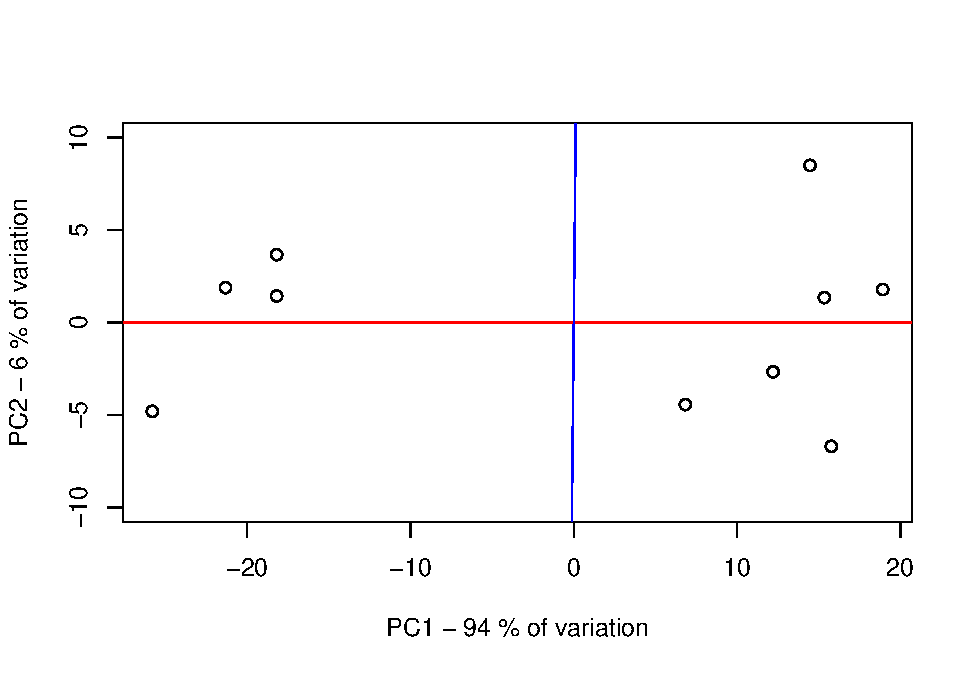
\includegraphics{Regresjon_Teori_files/figure-latex/unnamed-chunk-23-1.pdf}
\caption{Q-Q plott - `light-tail'}
\end{figure}

``Light-tailed'' (lette haler) har liten sannsynlighet for ekstreme
verdier og utvalg tenderer til å ikke fravike gjennomsnittet med mye.
Q-Q plottet for en fordeling med lette haler har ofte en S-form. Dataene
vokser saktere enn normalfordelingen i starten før den følger vekstraten
til normalfordelingen. Mot slutten vokser den raskere enn
normalfordelingen. Derfor bøyer den av fra normalfordelingen.

\hypertarget{bimodalitet}{%
\paragraph{Bimodalitet}\label{bimodalitet}}

\begin{figure}
\centering
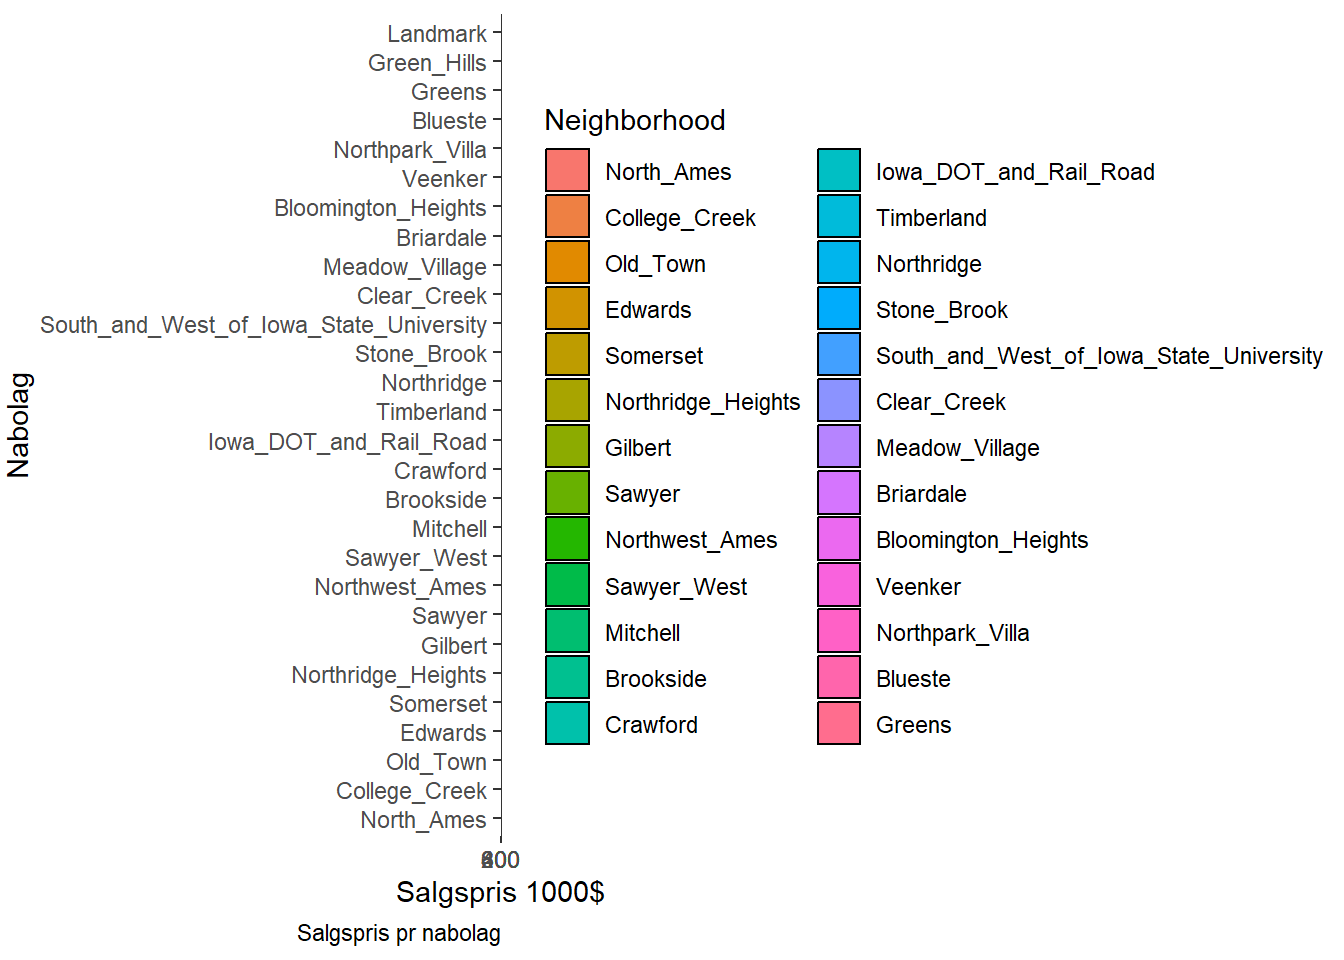
\includegraphics{Regresjon_Teori_files/figure-latex/unnamed-chunk-26-1.pdf}
\caption{Q-Q plott - bimodal}
\end{figure}

Den bimodiale fordelingen viser ofte et brudd eller et distinkt
knekkpunkt rundt krysning av den rette linja, med en del av linja på
hver side av den rette linja.

\hypertarget{multimodalitet}{%
\paragraph{Multimodalitet}\label{multimodalitet}}

\begin{figure}
\centering
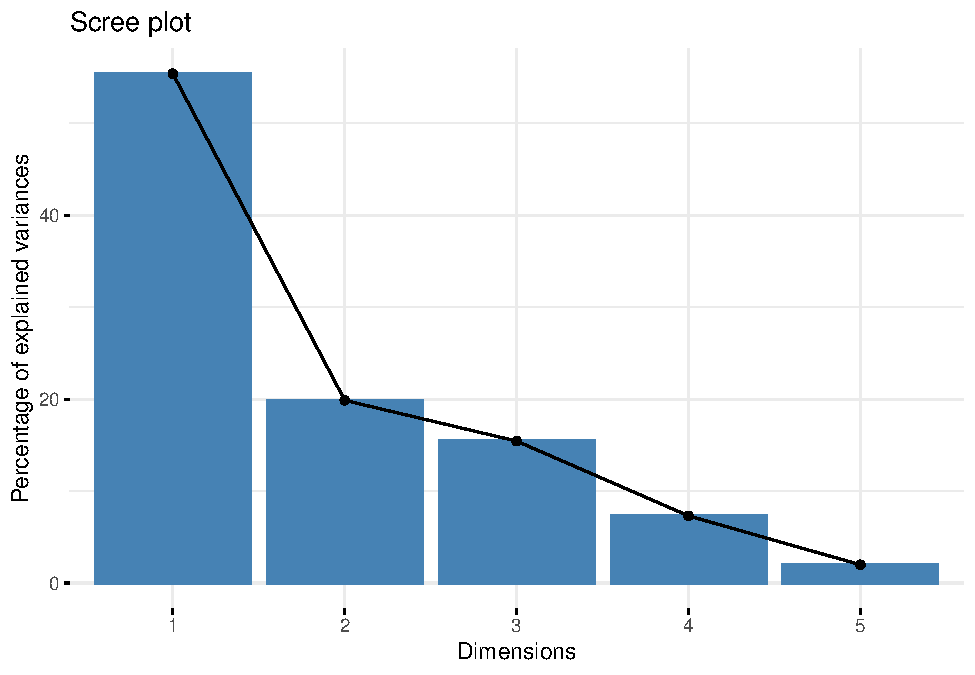
\includegraphics{Regresjon_Teori_files/figure-latex/unnamed-chunk-29-1.pdf}
\caption{Q-Q plott - multimodal}
\end{figure}

Multimodale fordelinger vil som regel vise flere brudd.

\hypertarget{statistiske-tester-for-vurdering-av-dataenes-distribusjon}{%
\subsubsection{Statistiske tester for vurdering av dataenes
distribusjon}\label{statistiske-tester-for-vurdering-av-dataenes-distribusjon}}

Vi har nå sett på noen typiske eksempler på mønstre i Q-Q plott. Det kan
imidlertid være vanskelig å bedømme fordelinger som ligger nære
normalfordelingen, men likevel ikke perfekt oppå (du vil trolig aldri se
en perfekt match med mindre du har generert et normalfordelt datasett
med mange datapunkter). Vi kan supplere Q-Q plottene med visse
statistiske tester (men husk: disse statistiske testene har sine egne
forutsetninger og er heller ikke uten utfordringer).

\hypertarget{anderson-darling}{%
\paragraph{Anderson-Darling}\label{anderson-darling}}

Anderson-Darlings test er en test for å se om et datasett kommer fra en
gitt fordeling, f.eks. normalfordelingen (Theodore W. Anderson and
Darling 1952; T. W. Anderson and Darling 1954). Testen setter opp to
hypoteser:

\begin{itemize}
\tightlist
\item
  \(H_0\): Dataene følger normalfordelingen
\item
  \(H_1\): Dataene følger ikke normalfordelingen
\end{itemize}

\begin{verbatim}
## 
##  Anderson-Darling normality test
## 
## data:  addata$Values
## A = 0.74573, p-value = 0.04046
\end{verbatim}

Siden vi vet at nullhypotesen er at datasettet \textbf{har} en
normalfordeling vil vi forkaste nullhypotesen dersom vi har en
signifikant p-verdi (grensen for hva som er signifikant bestemmer vi
forsåvidt selv, men vanlige verdier er 0.01, 0.05 og 0.1). Altså - i
dette tilfellet har vi en p-verdi=0.04. Vi forkaster derfor
nullhypotesen og aksepterer \(H_1\) som sier at dataene er trolig ikke
er normalfordelte (med andre ord: p-verdien må være større enn
signifikansverdien for at vi skal si at dataene trolig er
normalfordelte) - en huskeregel: ``If p is low, the null must go'' (her:
``low'' = under terskelverdien vi har satt, ofte 0.05).

Generisk ser dette slik ut (Hartmann, Krois, and Waske 2018):

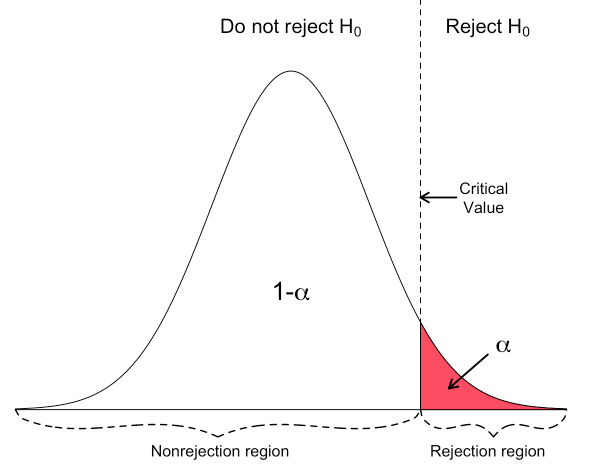
\includegraphics{Hartman1.png}

Det er verdt å merke seg at Anderson-Darling testen egentlig ikke
forteller deg at dataene dine er normalfordelte, men at det er
usannsynlig at de ikke er det om testen viser det. Dette synes kanskje
som samme sak, men er i realiteten en viktig erkjennelse -- en tørr
gressplen er et bevis for at det ikke har regnet, men en våt gressplen
er ikke bevis for at det har regnet. En våt gressplen kan skyldes andre
ting enn regn. Altså -- en signifikant p-verdi på testen gjør at vi
forkaster \(H_0\) og antar at fordelingen er ikke-normal. En
ikke-signifikant p-verdi på gjør at vi med f.eks. 95\% konfidens kan si
at vi ikke har funnet avvik fra normalfordelingen.

Tabellarisk kan vi oppsummere vurderingene slik:

\begin{table}[!h]
\centering
\begin{tabular}{l|l}
\hline
Betingelse & Vurdering\\
\hline
p-verdi $\le$ valgt signifikansnivå & Forkast $H_0$ - datene er trolig ikke normalfordelte\\
\hline
p-verdi > valgt signifikansnivå & Behold $H_0$ - dataene er trolig normalfordelte\\
\hline
Testverdi ($A^2$ verdi) > kritisk verdi & Forkast $H_0$ - datene er trolig ikke normalfordelte\\
\hline
Testverdi ($A^2$ verdi) $\le$ kritisk verdi & Behold $H_0$ - dataene er trolig normalfordelte\\
\hline
\end{tabular}
\end{table}

Det finnes flere andre statistiske tester som kan kjøres for å teste for
normalitet, f.eks. Kologorov-Smirnov, Shapiro-Wilks og Cramer Von-Mises
test. Vi går ikke inn på manuell utregning av disse i Excel.
Anderson-Darling er en modifisering/videreutvikling av
Kolmogorov-Smirnov og anses ofte som en bedre test av de to. Andre
kilder (se f.eks. Razali and Wah (2011)) finner at Shapiro-Wilks
presterer best i 10 000 simuleringer på ulike distribusjoner.

\begin{verbatim}
## 
##  One-sample Kolmogorov-Smirnov test
## 
## data:  addata5
## D = 0.88493, p-value = 0.0000000000000171
## alternative hypothesis: two-sided
\end{verbatim}

\begin{verbatim}
## 
##  Shapiro-Wilk normality test
## 
## data:  addata5$Values
## W = 0.87521, p-value = 0.04027
\end{verbatim}

\begin{verbatim}
## 
##  Cramer-von Mises normality test
## 
## data:  addata$Values
## W = 0.12634, p-value = 0.04326
\end{verbatim}

Tolkning Kolmogorov-Smirnov: Hvis p-verdien er under valgte
signifikansnivå (f.eks. 0.05) skal vi anta at datasettet ikke er
normalfordelt. Her vil testen peke på at datasettet \emph{ikke} er
normalfordelt.

Tolkning av Shapiro-Wilks og Cramer-von Mieses test er lik som for
Kolmogorov-Smirnov.

Som et siste eksempel på en statistisk test for normalitet kan vi bruke
Jarque-Bera test. Denne skiller seg litt ut fra de andre ved at den
spesifikt ser på skjevhet og kurtosis i datasettet opp mot hva en
normalfordeling vil ha. For å gjøre lykken komplett finnes det versjoner
av testen:

\begin{verbatim}
## 
##  Jarque Bera Test
## 
## data:  addata6$Values
## X-squared = 2.1953, df = 2, p-value = 0.3337
\end{verbatim}

\begin{verbatim}
## 
##  Adjusted Jarque-Bera test for normality
## 
## data:  addata6$Values
## AJB = 3.1014, p-value = 0.131
\end{verbatim}

Tolkningen er lik som før - hvis p-verdien er mindre enn valgte
signifikansnivå peker det mot at datasettet ikke er normalfordelt. Her,
i motsetning til de øvrige testene, er p-verdien større enn
signifikansnivået (0,05) så det peker mot at datasettet \emph{er}
normalfordelt.

Dette er altså ikke så enkelt. Det finnes mange statistiske tester, som
kan gi motsatte indikasjoner på om et datasett er normalfordelt eller
ikke siden de ser på dataene fra ``ulik vinkel'' (fokuserer på ulike
aspekter ved dataene). \textbf{Vårt råd blir:} Start alltid med Q-Q
plott. Velg evt en teststatistikk, men vær klar over at alle
teststatistikker bygger på forutsetninger eller tester ulike sider av
distribusjonen. Det vi også kan huske på er at i henhold til
sentralgrenseteoremet (``Central Limit Theorem'') vil populasjonens
fordeling være av mindre interesse dersom utvalgsstørrelsen er stor nok.
Hva er stor nok? De fleste kilder peker mot at over 30 er ``stort nok''.

\hypertarget{boxplott}{%
\subsubsection{Boxplott}\label{boxplott}}

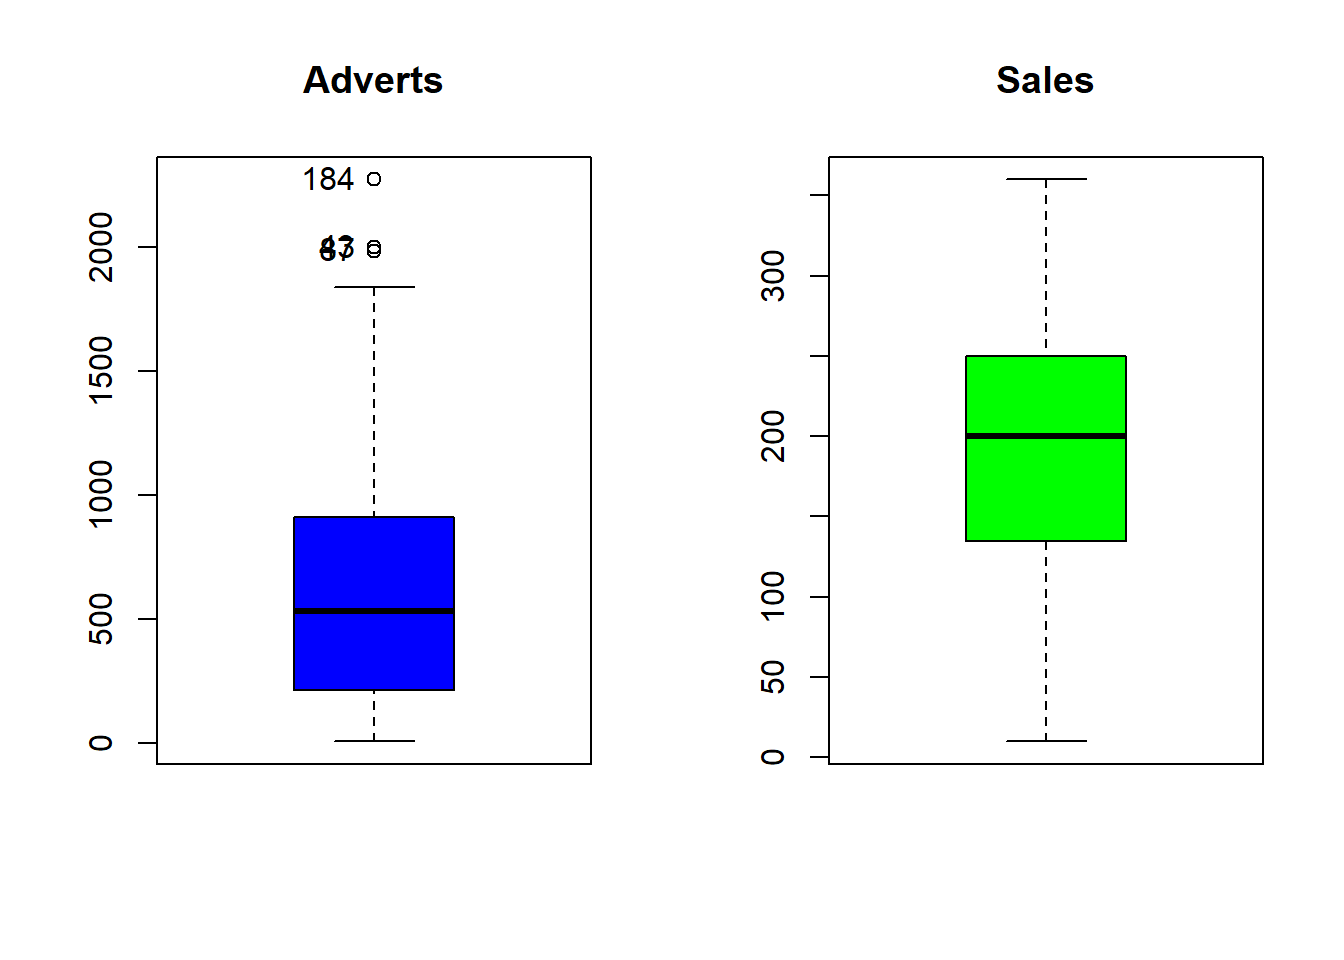
\includegraphics{Regresjon_Teori_files/figure-latex/unnamed-chunk-35-1.pdf}

Et boxplott forteller oss mye om dataenes distribusjon.

\begin{itemize}
\tightlist
\item
  Selve boksen representerer 50 \% av observasjonene/casene, det vil si
  at nedre kant representerer første kvartil (= 25.prosentil) og øvre
  kant tredje kvartil (= 75.prosentil).
\item
  Den tykkere horisontale streken i boksen viser medianverdien (= andre
  kvartil = 50.prosentil)
\item
  Dersom en observasjon ligger utenfor 1,5 x lengden på boksen vises
  dette med en liten sirkel. Dette defineres som uteliggere. Å
  identifisere uteliggere kan være viktig for mange statistiske tester.
\end{itemize}

Galarnyk (2018) illustrerer boxplott slik:

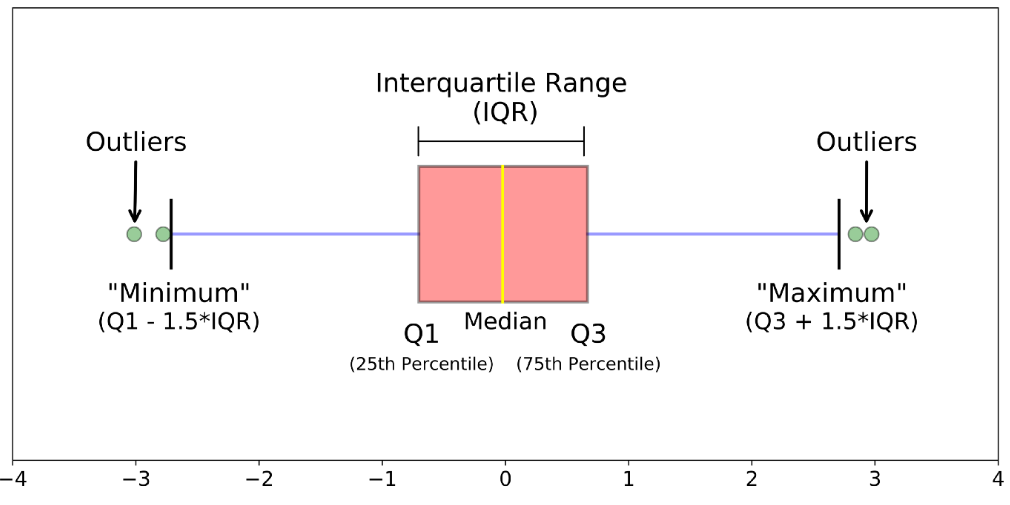
\includegraphics{Boxplott.png}

\hypertarget{scatterplott}{%
\subsubsection{Scatterplott}\label{scatterplott}}

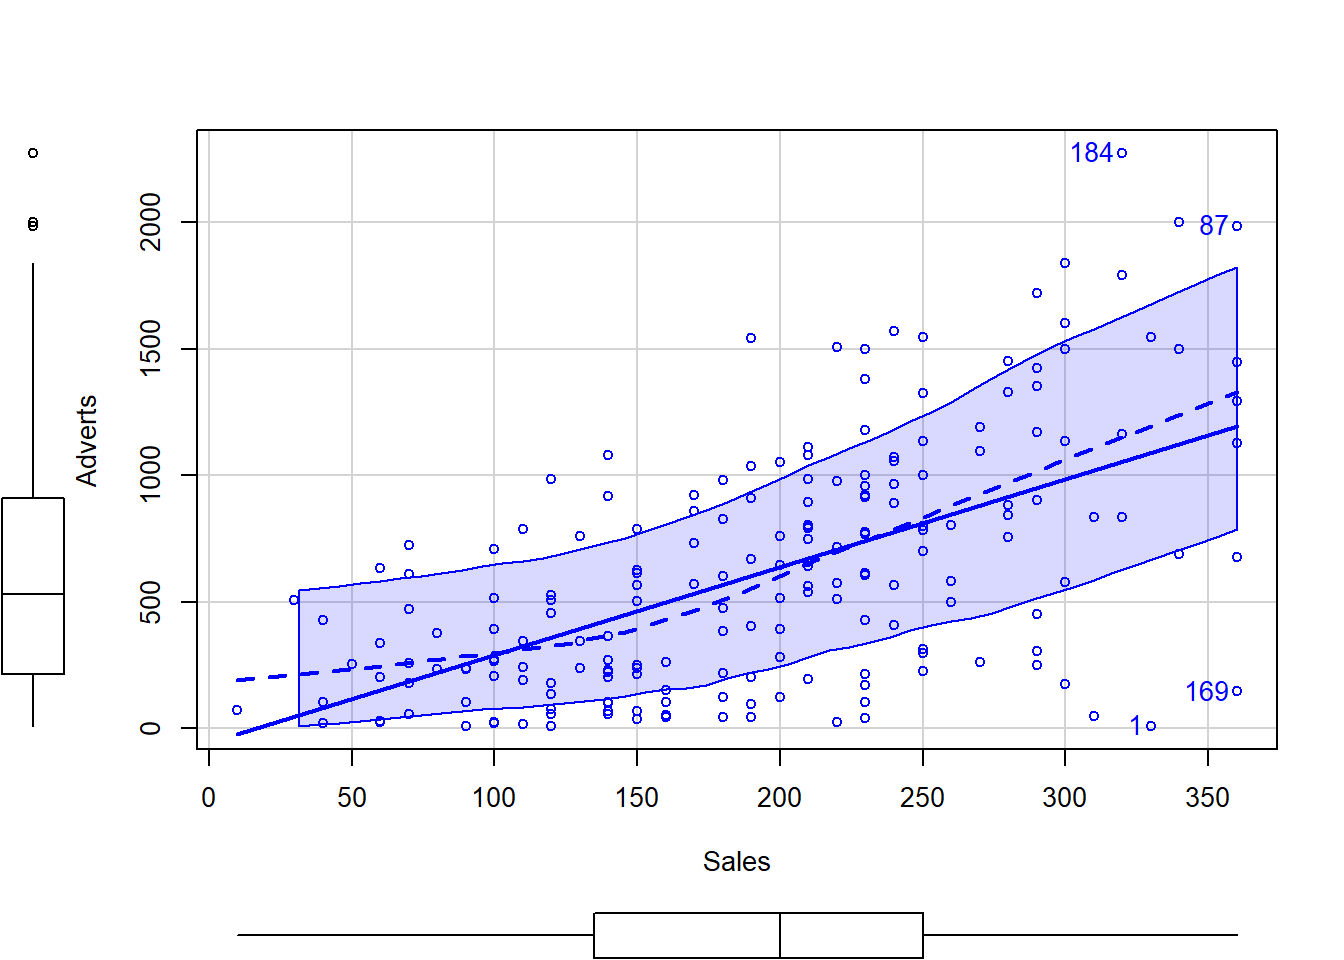
\includegraphics{Regresjon_Teori_files/figure-latex/unnamed-chunk-36-1.pdf}

Et scatterplott viser oss på en god visuell måte hvordan de to
variablene forholder seg til hverandre (vi plotter hver enkelt
observasjon gjennom verdiene de har på de to variablene). Mønsteret kan
derfor si oss mye om sammenhengen mellom de to.

En god måte å fremstille et scatterplott på i R (gjennom pakken
\emph{car}) er denne:
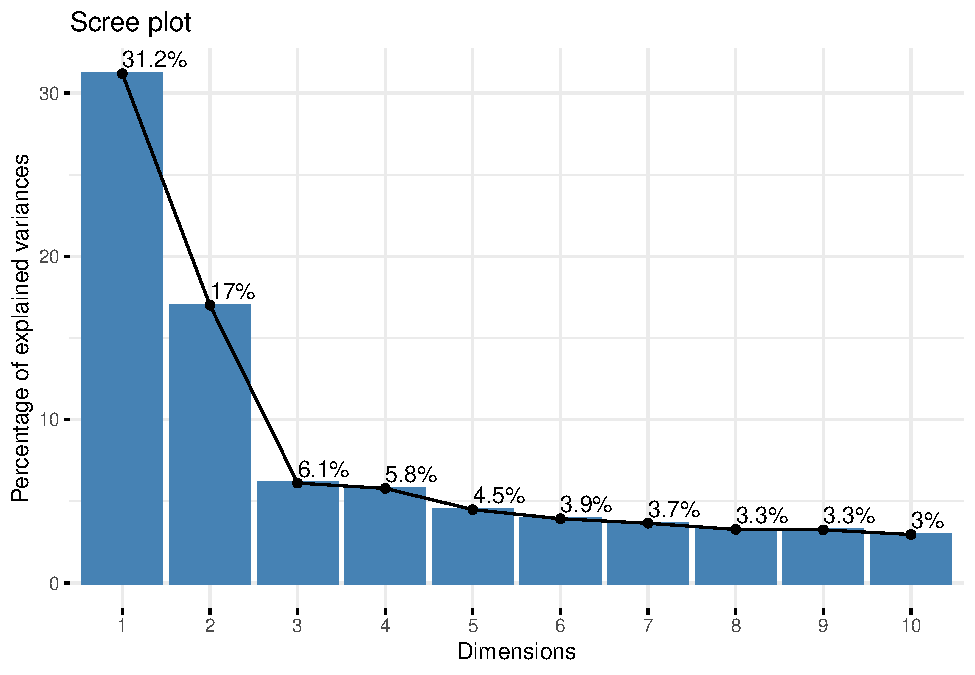
\includegraphics{Regresjon_Teori_files/figure-latex/unnamed-chunk-37-1.pdf}

\begin{verbatim}
## [1]   1  87 169 184
\end{verbatim}

Her kombinerer vi scatterplott og boxplott. Den rette blå linja er en
minste kvadratssums regresjonslinje (OLS). Den stiplede blå linja bruker
en ikke-parametrisk tilnærming. I tillegg får vi visualisert de fire
mest ekstreme tilfellene (lengst vekk fra gjennomsnitt).

\hypertarget{steg-2-evtentuelt-valg-av-prediktorer-ut-fra-analyse-av-dataene}{%
\subsection{Steg 2: Evtentuelt valg av prediktorer ut fra analyse av
dataene}\label{steg-2-evtentuelt-valg-av-prediktorer-ut-fra-analyse-av-dataene}}

Dette er ikke relevant i en enkel lineær regresjonsanalyse. Når vi skal
gjøre en multippel regresjonsanalyse - altså at vi har to eller flere
uavhengige variabler (prediktorer) vil analysen av dataene våre - og i
hvilken rekkefølge vi legger de uavhengige variablene inn i
regresjonsmodellen (mer om det under eksempelet for multippel regresjon)
kunne informeres av analysen vi gjør i forkant. Derfor viser vi dette nå
selv om det altså ikke er relevant for enkel regresjonsanalyse.

Vi lager en korrelasjonstabell for de tre uavhengige og den avhengige
variabelen (Sales, Adverts, Airplay, Image):

\begin{verbatim}
##            Adverts     Sales   Airplay      Image
## Adverts 1.00000000 0.5784877 0.1018828 0.08075151
## Sales   0.57848774 1.0000000 0.5989188 0.32611105
## Airplay 0.10188281 0.5989188 1.0000000 0.18198863
## Image   0.08075151 0.3261111 0.1819886 1.00000000
\end{verbatim}

I standard multippel regresjonsanalyse legger vi alle de uavhengige
variablene inn samtidig. Dersom vi skal gjøre en stegvis
regresjonsanalyse vil vi legge de uavhengige variablene inn en og en ut
fra statistiske kriterier - som hvor stor korrelasjonen er. Den
uavhengige variabelen med størst korrelasjon legges inn først og så
videre. For det eksempelet vi har ser vi at Sales korrelerer høyest med
Airplay, og nesten like mye med Adverts. Korrelasjonen med Image er noe
lavere.

\hypertarget{lage-modell-kjuxf8re-regresjonsanalysen}{%
\subsection{Lage modell (kjøre
regresjonsanalysen)}\label{lage-modell-kjuxf8re-regresjonsanalysen}}

Vi ønsker å se om Adverts kan predikere Sales. Grafisk kan vi vise
dette:

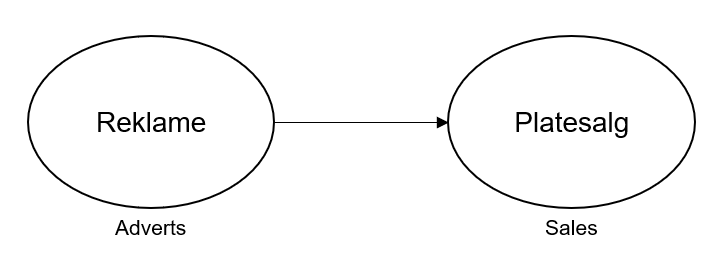
\includegraphics{OLS1.png}

\begin{verbatim}
## 
## Call:
## lm(formula = Sales ~ Adverts, data = Field_OLS)
## 
## Coefficients:
## (Intercept)      Adverts  
##   134.13994      0.09612
\end{verbatim}

\hypertarget{analyse-av-resultatene-diagnostikk}{%
\subsection{Analyse av resultatene
(diagnostikk)}\label{analyse-av-resultatene-diagnostikk}}

\begin{verbatim}
## 
## Call:
## lm(formula = Sales ~ Adverts, data = Field_OLS)
## 
## Residuals:
##      Min       1Q   Median       3Q      Max 
## -152.949  -43.796   -0.393   37.040  211.866 
## 
## Coefficients:
##               Estimate Std. Error t value            Pr(>|t|)    
## (Intercept) 134.139938   7.536575  17.799 <0.0000000000000002 ***
## Adverts       0.096124   0.009632   9.979 <0.0000000000000002 ***
## ---
## Signif. codes:  0 '***' 0.001 '**' 0.01 '*' 0.05 '.' 0.1 ' ' 1
## 
## Residual standard error: 65.99 on 198 degrees of freedom
## Multiple R-squared:  0.3346, Adjusted R-squared:  0.3313 
## F-statistic: 99.59 on 1 and 198 DF,  p-value: < 0.00000000000000022
\end{verbatim}

\hypertarget{hvor-mye-forklarer-modellen-vuxe5r}{%
\subsubsection{Hvor mye forklarer modellen
vår?}\label{hvor-mye-forklarer-modellen-vuxe5r}}

Det første vi kan se på er \(R^{2}\) som forteller oss hvor stor del av
den totale variansen modellen forklarer. I dette tilfellet er \(R^{2}\)
= 0.3346. Det innebærer at modellen vår kan forklare 33.46 \% av den
totale variansen. Det betyr at reklame forklarer («accounts for») 33.5
\% av variansen i salget. Det er med andre ord mange andre faktorer som
kan forklare hvorfor noen plater selger bedre enn andre, men reklame kan
forklare drøye 33 \% av den totale variansen. Dette kan vi også se er
statistisk signifikant p \textless{} .001.

Endel programmer vil også gi en R verdi. Siden vi kun har en uavhengig
variabel (en prediktor) vil verdien R utgjøre den bivariate
korrelasjonen (korrelasjonskoeffisienten mellom de to variablene - vi
ser at dette er samme verdi som i tabellen over
korrelasjonskoeffisienter lenger opp).

Adjusted \(R^{2}\) er en ``modifisert versjon'' av \(R^{2}\) der det
legges inn en korreksjon for antall prediktorer i modellen. Motivasjonen
for dette er at det å legge til flere prodeiktorer \emph{alltid} vil øke
\(R^{2}\) verdien (Navarro and Foxcroft 2019). Navarro and Foxcroft
(2019) påpeker imidlertid at man ikke kan tolke adjusted \(R^{2}\) like
rett fram som \(R^{2}\), og anbefaler at man bruker \(R^{2}\). Det vi
også kan si er at dersom verdiene på henholdsvis \(R^{2}\) og adjusted
\(R^{2}\) er nærme hverandre (eller like) indikerer dette en god
kryssvaliditet i modellen, noe som kan gjøre oss sikrere i
generalisering av funnene våre.

\hypertarget{modellens-koeffisienter-og-regresjonslikning}{%
\subsubsection{Modellens koeffisienter og
regresjonslikning}\label{modellens-koeffisienter-og-regresjonslikning}}

Koeffisientene vil fortelle oss mer i multippel regresjonsanalyse, men
gir oss noen interessante opplysninger også her. I introduksjonen
snakket vi om punktet der regresjonslinja skjærer y-aksen (konstanten).
Fra analysen ser vi at (Intercept) = 134.14 og Adverts = 0.096. 134.14
er punktet på y-aksen regresjonslinja ``begynner'' (der x = 0). Altså,
ettersom x-aksen angir verdier for hva vi bruker på reklame er Intercept
estimatet antallet plater vi kan forvente å selge dersom vi bruker 0
kroner på reklame. Estimatet på «Adverts» på 0,096 er stigningstallet
for regresjonslinja -- hvis prediktoren (reklame) stiger med 1 enhet
stiger salget med 0,096 plater. Vi kan da lage følgende likning:
\[ Sales=134,14\:+\:0,096\left(Adverts\right) \]

\hypertarget{hvor-god-er-modellen-vuxe5r-goodness-of-fit}{%
\subsubsection{Hvor god er modellen vår (goodness of
fit)?}\label{hvor-god-er-modellen-vuxe5r-goodness-of-fit}}

Vi ønsker å ha en formening om hvor god modellen er («goodness of fit»).
Altså, er regresjonsmodellen vår bedre enn en modell der vi ikke vet noe
om forholdet mellom reklame og platesalg? Vi kan bruke gjennomsnitt av
salgstallene som en modell for ingen sammenheng mellom reklame og
platesalg, og deretter sammenlikne regresjonsmodellen med
gjennomsnittsmodellen. Sammenlikningen mellom modellene skjer gjennom å
se på forskjellene mellom de observerte målingene (salgstall) og verdier
predikert at de to ulike modellene. Dersom regresjonsmodellen
signifikant predikerer bedre er det en bedre modell enn alternativet.

Analysen vår gitt oss F verdien 99.59 med p \textless{} .001. Vi ser at
verdien er statistisk signifikant. F verdien er et mål på forbedring i
prediksjonen sett opp mot unøyaktigheter i modellen (alle modeller er
unøyaktige (eller ``feil'')). Vi kan sjekke F-verdien opp mot antall
frihetsgrader (df) gjennom tabeller som ofte finnes i statistikkbøker,
eller bruke onlineressurser som her:
\href{http://www.stat.purdue.edu/~jtroisi/STAT350Spring2015/tables/FTable.pdf}{her}

Vi ser av resultatene fra analysen at antall df i teller er 1 og antall
df i nevner er 198. Hvis vi leser av tabellen er vi at for df 1/df 200
er kritisk verdi 3,89 for α = 0,05 og 11,15 for α = 0,001. Vår F er med
andre ord langt over kritisk verdi. Vi kan derfor si at vår
regresjonsmodell gir en signifikant bedre prediksjon av platesalg enn
alternativet. Reklame er med andre ord en god prediktor for platesalg.

Helt nøyaktig kan vi regne ut kritisk verdi (som vi har gjort i R) for
df 1 og df 198:

\begin{verbatim}
## [1] 3.888853
\end{verbatim}

Ut fra dette kan vi si det er svært usannsynlig at forbedringen fra
referansemodellen (gjennomsnittet) til vår modell er tilfeldig. Vi kan
også si at dersom forbedringen ved regresjonsmodellen er større enn
unøyaktigheten i modellen så vil F \textgreater{} 1.

Til slutt vil vi se på konfidensintervallet:

\begin{verbatim}
##                 Estimate        2.5 %      97.5 %
## (Intercept) 134.13993781 119.27768082 149.0021948
## Adverts       0.09612449   0.07712929   0.1151197
\end{verbatim}

\hypertarget{sjekk-av-forutsetningene}{%
\subsection{Sjekk av forutsetningene}\label{sjekk-av-forutsetningene}}

Dette er et tema som behandles og framstilles på noe ulike måter i
litteraturen. Det som er klart er at brudd på forutsetningene \emph{kan}
gjøre modellen vår mer usikker opp til et punkt hvor regresjonsanalyse
ikke bør gjennomføres. Noen av forutsetningene er empirisk testbare (vi
kan få ut en eller annen form for analyse av et statistikkprogram som
SPSS, Stata, R og så videre) mens noen er ikke empirisk testbare (det
vil si vi må bruke egen vurdering). Vi skal i dette delkapittelet gå
gjennom forutsetningene for lineær regresjon. Selv om noen ikke er
aktuelle for enkel regresjon tar vi med alle forutsetningene her for
oversiktens skyld.

Ved regresjonsanalyse gjør vi en rekke sjekker av datamaterialet vi har
for å avgjøre om regresjonsanalyse er en egnet teknikk og hvorvidt vi
mener vi kan generalisere funnene. Dersom forutsetningene brytes gjør
det at vi kan sette spørsmålstegn ved hvor nærme regresjonskoeffisienten
er populasjonskoeffisienten -- eller med andre ord: Hvis
regresjonskoeffisienten er helt forventningsrett («unbiased», dvs 0) så
vil regresjonskoeffisienten være lik populasjonskoeffisienten
(«estimatet er lik virkeligheten»). Nå vil det i praksis aldri være
tilfelle, men ved å sette visse forutsetninger kan vi fastslå om våre
data egner seg for regresjonsanalyse og hvor sikre vi føler oss for at
funnene kan generaliseres. Det er verdt å merke seg hva Field et. al
(2012, s.298) skriver:

\begin{quote}
``It's worth remembering that you can have a perfectly good model for
your data (no outliers, influential cases, etc.) and you can use that
model to draw conclusions about your sample, even if your assumptions
are violated. However, it's much more interesting to generalize your
regression model and this is where assumptions become important. If they
have been violated then you cannot generalize your findings beyond your
sample.''
\end{quote}

Med andre ord: Vi kan ha brudd på forutsetningene og likevel si noe
meningsfullt om vårt utvalg/våre data, men resultatene våre blir mer
usikre og vi skal være veldig forsiktige med å kreve generaliserbarhet
dersom vi har brudd på forutsetningene. Så alt håp er ikke ute med brudd
på forutsetningene, men vi skal behandle konklusjonene våre deretter.

Regresjonsforutsetninger behandles ulikt av ulke kilder, og får ulik
plass i diskusjoner om regresjon. Vi har undersøkt en rekke kilder for å
framstille dette her (blant annet Green (1991), Berry (1993), Miles and
Shevlin (2001), Hinkle, Wiersma, and Jurs (2003), Tabachnik and Fidell
(2007), Eikemo and Clausen (2007), Hair Jr. et al. (2010), Lomax and
Hahs-Vaughn (2012)).

Vi vil i det følgende ta utgangspunkt i Thrane (2019)'s inndeling i tre
hovedkateogrier (vi velger å utvide Thranes punkter med det vi mener er
et par relevante tillegg).

\begin{enumerate}
\def\labelenumi{\arabic{enumi}.}
\tightlist
\item
  Ikke-testbare forutsetninger
\item
  Testbare forutsetninger som ikke krever tilfeldig utvalg
\item
  Testbare forutsetninger for et tilfeldig utvalg
\end{enumerate}

\hypertarget{ikke-testbare-forutsetninger}{%
\subsubsection{Ikke-testbare
forutsetninger}\label{ikke-testbare-forutsetninger}}

\hypertarget{kausalitet}{%
\paragraph{Kausalitet}\label{kausalitet}}

Forutsetningen om kausalitet hviler i fagunnskap og teoretiske
vurderinger. Det sier seg for så vidt selv at vi ikke er interesserte i
å ha med irrelevante variabler i modellen. Med irrelevant her menes
variabler som korrelerer med den avhengige variabelen, men hvor
korrelasjonen er ikke har noe med årsakssammenheng å gjøre (sammenhenger
medfører ikke i seg selv kausalitet som vi har vært inne på i en
tidligere modul).

Kausalitet er dermed en forutsetning. Den uavhengige variabelen må
variere korrelert med de avhengige, det er en kausal sammenheng (hvis
ikke det er kausalitet har den/de uavhengige variablene ingen effekt på
den avhengige -- det kan like gjerne være motsatt). Når vi velger en
avhengig variabel og en eller flere uavhengige variabler har vi også
gjort en antakelse om kausalitet og retning på kausaliteten, og
forutsatt at denne er tilstede - basert på teoretisk kunnskap om det vi
undersøker. Men det er viktig å understreke at verken korrelasjon eller
regresjon indikerer kausalitet.

\hypertarget{variablene-er-uten-muxe5lefeil}{%
\paragraph{Variablene er uten
målefeil}\label{variablene-er-uten-muxe5lefeil}}

Vi må forutsette at vi ikke har systematiske målefeil i våre data.
Thoresen (2003) viser for eksempel til en studie av MacMahon et al.
(1990) der de fant en 60\% sterkere sammneheng mellom blodtrykk og
hjerte-karsykdommer i en stor metastudie når de korrigerte for skjevhet
i estimatene i de tidligere studiene (som var inkludert i metastudien).

Vi skal også være oppmerksom på utfordringer dersom feil i den ene
variabelen korrelerer med feil i en annen variabel. ``Dersom målt
eksponering og målt helseutfall er rammet av avhengige feil, blir
resultatet oftest en falskt forhøyet sammenheng mellom de to. Slik
resultatskjevhet er sannsynligvis ikke uvanlig i tverrsnittsstudier,
hvor data om eksponering og utfall skaffes til veie gjennom
spørreskjema'' (Kristensen 2005).

\hypertarget{relevante-og-irrelevante-variabler}{%
\paragraph{Relevante og irrelevante
variabler}\label{relevante-og-irrelevante-variabler}}

Alle relevante uavhengige variabler må være inkludert i modellen, og
alle irrelevante uvhengige variabler er fjernet/er ikke med i modellen.
Man kan si at en hovedgrunn til at vi veldig ofte kjører mulitippel
regresjonsanalyse i stedet for bivariat regresjonsanalyse er for å unngå
at vi ikke inkluderer relevante variabler (såkalt ``omitted variable
bias'') (Thrane 2019). Imidlertid, som Thrane (2019) påpeker, er dette i
praksis umulig, så det vi tilstrebe er å inkludere de mest relevante
variablene. Dette faller igjen tilbake på teoretiske betraktninger og
faglig kjennskap til området man holder på med. Du skal i hvert fall
kunne begrunne valget av hvilke uavhengige variabler som er inkludert og
hvilke som kanskje kunne tenkes å være inkludert, men som du har valgt å
ikke inkludere.

Teoretisk sett skal vi også forsikre oss om at ikke-relevante variabler
ikke er inkludert i modellen. Igjen er dette delvis umulig og delvis
forvirrende/unøyaktig. Det er delvis umulig fordi vi vanskelig kan vite
eksakt hvilke potensielle variabler som er relevante og ikke. Det er
delvis forvirrende/unøyaktig fordi det kan være viktig å identifisere
variabler som ikke har noen effekt - dette kan være viktig i
policyrevisjon/-utforming (jfr Thrane (2019)).

\hypertarget{testbare-forutsetninger-som-ikke-krever-tilfeldig-utvalg}{%
\subsubsection{Testbare forutsetninger som ikke krever tilfeldig
utvalg}\label{testbare-forutsetninger-som-ikke-krever-tilfeldig-utvalg}}

\hypertarget{forholdstall-mellom-caserobservasjoner-og-uavhengige-variabler}{%
\paragraph{Forholdstall mellom caser/observasjoner og uavhengige
variabler}\label{forholdstall-mellom-caserobservasjoner-og-uavhengige-variabler}}

Forholdstallet mellom respondenter/caser/observasjoner og uavhengig
variabler er av stor betydning dersom man skal gjennomføre en multippel
regresjon. Dette gjelder spesielt ved skjevdistribusjon av den avhengige
variabelen, effektstørrelsen er forventet liten eller man kan mistenke
vesentlige målefeil (Tabachnik and Fidell 2007).

Det finnes ulike anbefalte normer for vurdering av forholdstallet (vi
tar her utgangspunkt i standard multippel regresjonsanalyse - stegvis
multippel regresjonsanalyse kan gi andre vurderinger rundt
forholdstallet). Under viser vi noen eksempler på hvordan man kan
vurdere dette:

\providecommand{\docline}[3]{\noalign{\global\setlength{\arrayrulewidth}{#1}}\arrayrulecolor[HTML]{#2}\cline{#3}}

\setlength{\tabcolsep}{2pt}

\renewcommand*{\arraystretch}{1.5}

\begin{longtable}[c]{|p{2.50in}|p{4.50in}}

\caption{Forholdstall
}\\

\hhline{>{\arrayrulecolor[HTML]{666666}\global\arrayrulewidth=2pt}->{\arrayrulecolor[HTML]{666666}\global\arrayrulewidth=2pt}-}

\multicolumn{1}{!{\color[HTML]{000000}\vrule width 0pt}>{\cellcolor[HTML]{ADDFAD}\raggedright}p{\dimexpr 2.5in+0\tabcolsep+0\arrayrulewidth}}{\fontsize{11}{11}\selectfont{\textcolor[HTML]{000000}{\textbf{Kilde}}}} & \multicolumn{1}{!{\color[HTML]{000000}\vrule width 0pt}>{\cellcolor[HTML]{ADDFAD}\raggedright}p{\dimexpr 4.5in+0\tabcolsep+0\arrayrulewidth}!{\color[HTML]{000000}\vrule width 0pt}}{\fontsize{11}{11}\selectfont{\textcolor[HTML]{000000}{\textbf{Antall}}}} \\

\hhline{>{\arrayrulecolor[HTML]{666666}\global\arrayrulewidth=2pt}->{\arrayrulecolor[HTML]{666666}\global\arrayrulewidth=2pt}-}

\endfirsthead

\hhline{>{\arrayrulecolor[HTML]{666666}\global\arrayrulewidth=2pt}->{\arrayrulecolor[HTML]{666666}\global\arrayrulewidth=2pt}-}

\multicolumn{1}{!{\color[HTML]{000000}\vrule width 0pt}>{\cellcolor[HTML]{ADDFAD}\raggedright}p{\dimexpr 2.5in+0\tabcolsep+0\arrayrulewidth}}{\fontsize{11}{11}\selectfont{\textcolor[HTML]{000000}{\textbf{Kilde}}}} & \multicolumn{1}{!{\color[HTML]{000000}\vrule width 0pt}>{\cellcolor[HTML]{ADDFAD}\raggedright}p{\dimexpr 4.5in+0\tabcolsep+0\arrayrulewidth}!{\color[HTML]{000000}\vrule width 0pt}}{\fontsize{11}{11}\selectfont{\textcolor[HTML]{000000}{\textbf{Antall}}}} \\

\hhline{>{\arrayrulecolor[HTML]{666666}\global\arrayrulewidth=2pt}->{\arrayrulecolor[HTML]{666666}\global\arrayrulewidth=2pt}-}\endhead



\multicolumn{1}{!{\color[HTML]{000000}\vrule width 0pt}>{\raggedright}p{\dimexpr 2.5in+0\tabcolsep+0\arrayrulewidth}}{\fontsize{11}{11}\selectfont{\textcolor[HTML]{000000}{Marks\ (1966,\ i\ Harris\ (2013)}}} & \multicolumn{1}{!{\color[HTML]{000000}\vrule width 0pt}>{\raggedright}p{\dimexpr 4.5in+0\tabcolsep+0\arrayrulewidth}!{\color[HTML]{000000}\vrule width 0pt}}{\fontsize{11}{11}\selectfont{\textcolor[HTML]{000000}{Minimum\ 200\ uansett}}} \\

\hhline{>{\arrayrulecolor[HTML]{666666}\global\arrayrulewidth=0.5pt}->{\arrayrulecolor[HTML]{666666}\global\arrayrulewidth=0.5pt}-}



\multicolumn{1}{!{\color[HTML]{000000}\vrule width 0pt}>{\raggedright}p{\dimexpr 2.5in+0\tabcolsep+0\arrayrulewidth}}{\fontsize{11}{11}\selectfont{\textcolor[HTML]{000000}{Schmidt\ (1971)}}} & \multicolumn{1}{!{\color[HTML]{000000}\vrule width 0pt}>{\raggedright}p{\dimexpr 4.5in+0\tabcolsep+0\arrayrulewidth}!{\color[HTML]{000000}\vrule width 0pt}}{\fontsize{11}{11}\selectfont{\textcolor[HTML]{000000}{15-1\ til\ 25-1}}} \\

\hhline{>{\arrayrulecolor[HTML]{666666}\global\arrayrulewidth=0.5pt}->{\arrayrulecolor[HTML]{666666}\global\arrayrulewidth=0.5pt}-}



\multicolumn{1}{!{\color[HTML]{000000}\vrule width 0pt}>{\raggedright}p{\dimexpr 2.5in+0\tabcolsep+0\arrayrulewidth}}{\fontsize{11}{11}\selectfont{\textcolor[HTML]{000000}{Nunally\ (1978)}}} & \multicolumn{1}{!{\color[HTML]{000000}\vrule width 0pt}>{\raggedright}p{\dimexpr 4.5in+0\tabcolsep+0\arrayrulewidth}!{\color[HTML]{000000}\vrule width 0pt}}{\fontsize{11}{11}\selectfont{\textcolor[HTML]{000000}{2-3\ IV\ =\ minst\ 100,\ 9-10\ IV\ =\ 300-400}}} \\

\hhline{>{\arrayrulecolor[HTML]{666666}\global\arrayrulewidth=0.5pt}->{\arrayrulecolor[HTML]{666666}\global\arrayrulewidth=0.5pt}-}



\multicolumn{1}{!{\color[HTML]{000000}\vrule width 0pt}>{\raggedright}p{\dimexpr 2.5in+0\tabcolsep+0\arrayrulewidth}}{\fontsize{11}{11}\selectfont{\textcolor[HTML]{000000}{Stevens\ (1996)}}} & \multicolumn{1}{!{\color[HTML]{000000}\vrule width 0pt}>{\raggedright}p{\dimexpr 4.5in+0\tabcolsep+0\arrayrulewidth}!{\color[HTML]{000000}\vrule width 0pt}}{\fontsize{11}{11}\selectfont{\textcolor[HTML]{000000}{15\ pr\ IV}}} \\

\hhline{>{\arrayrulecolor[HTML]{666666}\global\arrayrulewidth=0.5pt}->{\arrayrulecolor[HTML]{666666}\global\arrayrulewidth=0.5pt}-}



\multicolumn{1}{!{\color[HTML]{000000}\vrule width 0pt}>{\raggedright}p{\dimexpr 2.5in+0\tabcolsep+0\arrayrulewidth}}{\fontsize{11}{11}\selectfont{\textcolor[HTML]{000000}{Green\ (1991)}}} & \multicolumn{1}{!{\color[HTML]{000000}\vrule width 0pt}>{\raggedright}p{\dimexpr 4.5in+0\tabcolsep+0\arrayrulewidth}!{\color[HTML]{000000}\vrule width 0pt}}{\fontsize{11}{11}\selectfont{\textcolor[HTML]{000000}{N=50+8m\ (m=antall\ uavhengige\ variabler)\ ved\ «medium-sized\ relationship\ between\ the\ IVs\ and\ the\ DV,\ a=.05\ and\ ß=.20}}} \\

\hhline{>{\arrayrulecolor[HTML]{666666}\global\arrayrulewidth=0.5pt}->{\arrayrulecolor[HTML]{666666}\global\arrayrulewidth=0.5pt}-}



\multicolumn{1}{!{\color[HTML]{000000}\vrule width 0pt}>{\raggedright}p{\dimexpr 2.5in+0\tabcolsep+0\arrayrulewidth}}{\fontsize{11}{11}\selectfont{\textcolor[HTML]{000000}{Miles\ \&\ Shevlin\ (2001)}}} & \multicolumn{1}{!{\color[HTML]{000000}\vrule width 0pt}>{\raggedright}p{\dimexpr 4.5in+0\tabcolsep+0\arrayrulewidth}!{\color[HTML]{000000}\vrule width 0pt}}{\fontsize{11}{11}\selectfont{\textcolor[HTML]{000000}{Som\ Green\ (2001).\ Utvalgsstørrelse\ avhenger\ av\ størrelse\ på\ effekt\ og\ statistisk\ styrke\ (se\ Cohen,\ 1988\ for\ effektstørrelser).\ Stor\ effekt:\ 80\ respondenter\ er\ alltid\ nok\ for\ opptil\ 20\ IVs.\ Middels\ effekt:\ 200\ respondenter\ vil\ alltid\ være\ nok\ for\ opptil\ 20\ IVs,\ 100\ er\ nok\ for\ opptil\ 6\ eller\ færre\ IVs.\ Lav\ effekt:\ Minst\ 600.}}} \\

\hhline{>{\arrayrulecolor[HTML]{666666}\global\arrayrulewidth=2pt}->{\arrayrulecolor[HTML]{666666}\global\arrayrulewidth=2pt}-}



\end{longtable}

Det er også verdt å merke seg at det ikke er ønskelig med for mange
respondenter, da et svært stort antall respondenter vil gi statistisk
signifikans for nesten enhver multippel korrelasjon -- ``For both
statistical and practical reasons, then, one wants to measure the
smallest number of cases that has a decent chance of revealing a
relationship of a specified size'' (Tabachnik and Fidell 2007, s.123).
Dette har med andre ord mye å si for hvordan man planlegger en studie.
Miles and Shevlin (2001), som angitt i siste rad i tabellen over, ser på
sammenhengen mellom effektstørrelse, statistisk styrke og
utvalgsstørrelse. Field (2009, s.223, figur 7.10) har modifisert grafisk
denne sammenhengen:

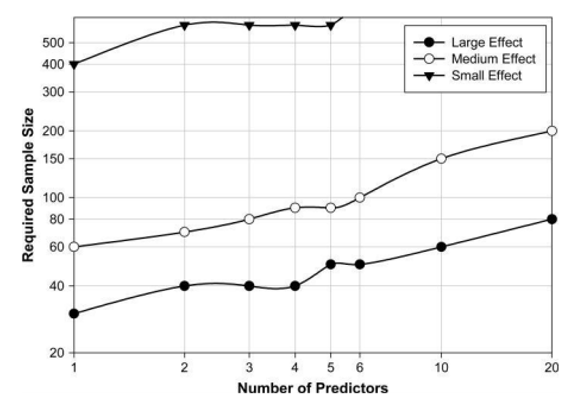
\includegraphics{Field_s223.png}

\hypertarget{dende-uavhengige-variablen-er-additiv-for-den-avhengige-variabelen}{%
\paragraph{Den(de) uavhengige variablen er additiv for den avhengige
variabelen}\label{dende-uavhengige-variablen-er-additiv-for-den-avhengige-variabelen}}

Med dette menes at vi må forvente at variasjonen i den avhengige
variabelen er en funksjon av sum av endringer i den/de uavhengige
variablen(e).

\hypertarget{linearitet}{%
\paragraph{Linearitet}\label{linearitet}}

Vi tar, som navnet ``linær regresjonsanalyse'' ganske klart indikerer,
utgangspunkt i at forholdet mellom den/de uavhengige varaibelen(e) og
den avhengige variabelen kan beskrives som en lineær funksjon (se for
eksempel Ringdal (2007)). Sammenhengen mellom variablene må ikke være
perfekt lineær, men må i hvert fall være tilnærmet lineær.

Vi har allerede sett en grafisk framstilling under punktet analyse av
dataene som lar oss visuelt vurdere denne forutsetningen:

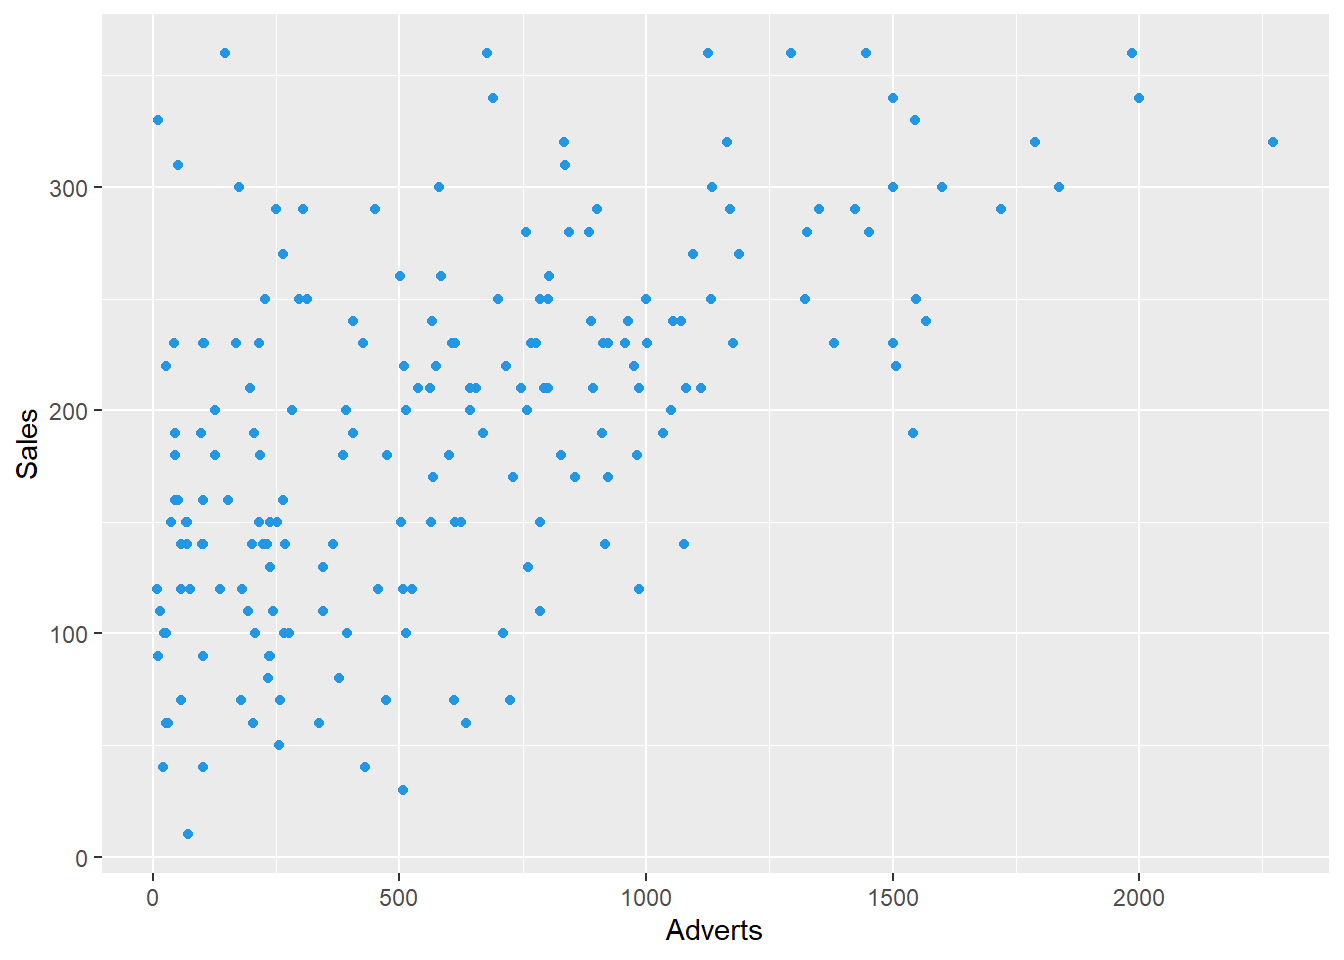
\includegraphics{Regresjon_Teori_files/figure-latex/unnamed-chunk-45-1.pdf}

Den stiplede linjen som buer ca midt i det skraverte området gjør ingen
forutsetninger, men plotter bare dataene (ofte kalt ``scatterplot
smoother''). Vi kan vurdere om denne er nærme eller langt fra en rett
linje. I grafen over ligger det både en stiplet buet linje og en rett
linje (regresjonslinje). I vårt tilfelle vil vi raskt konkludere med at
forholdet mellom de to variablene er tilnærmet lineært.

\hypertarget{fravuxe6r-av-multkolinearitet}{%
\paragraph{Fravær av
multkolinearitet}\label{fravuxe6r-av-multkolinearitet}}

\hypertarget{eventuell-revisjon-av-modell}{%
\subsection{Eventuell revisjon av
modell}\label{eventuell-revisjon-av-modell}}

Her kan vi for eksempel se hvordan modellens presterer ved bortfall av
visse ektreme verdier (uteliggere) eller ved inkludering/eksklusjon av
gitte variabler i modellen (først og fremst ved multippel
regresjonsanalyse).

Vi så under punktet ``Analyse av dataene'' (se for eksempel Boxplottet
av Adverts) at vi har noen observasjoner i modellen som kan defineres
som uteliggere. Vi kan identifisere disse gjennom residualene:

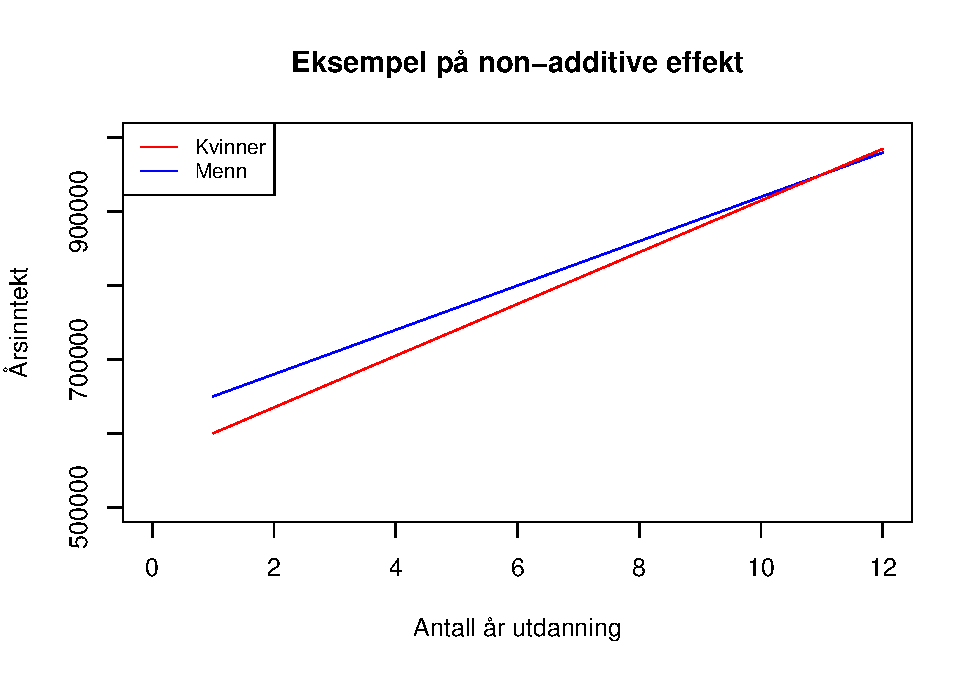
\includegraphics{Regresjon_Teori_files/figure-latex/unnamed-chunk-46-1.pdf}

\begin{verbatim}
## [1]   1  42 169
\end{verbatim}

Vi ser at residualene, med unntak av observasjonene 42 (som ligger
utenfor 95\% konfidenstintervall - boostrapped) og 1 som ligger på
grensen.

Vi kan også kjøre en analyse som identifiserer betydning/innvirkning
(``influential cases''):

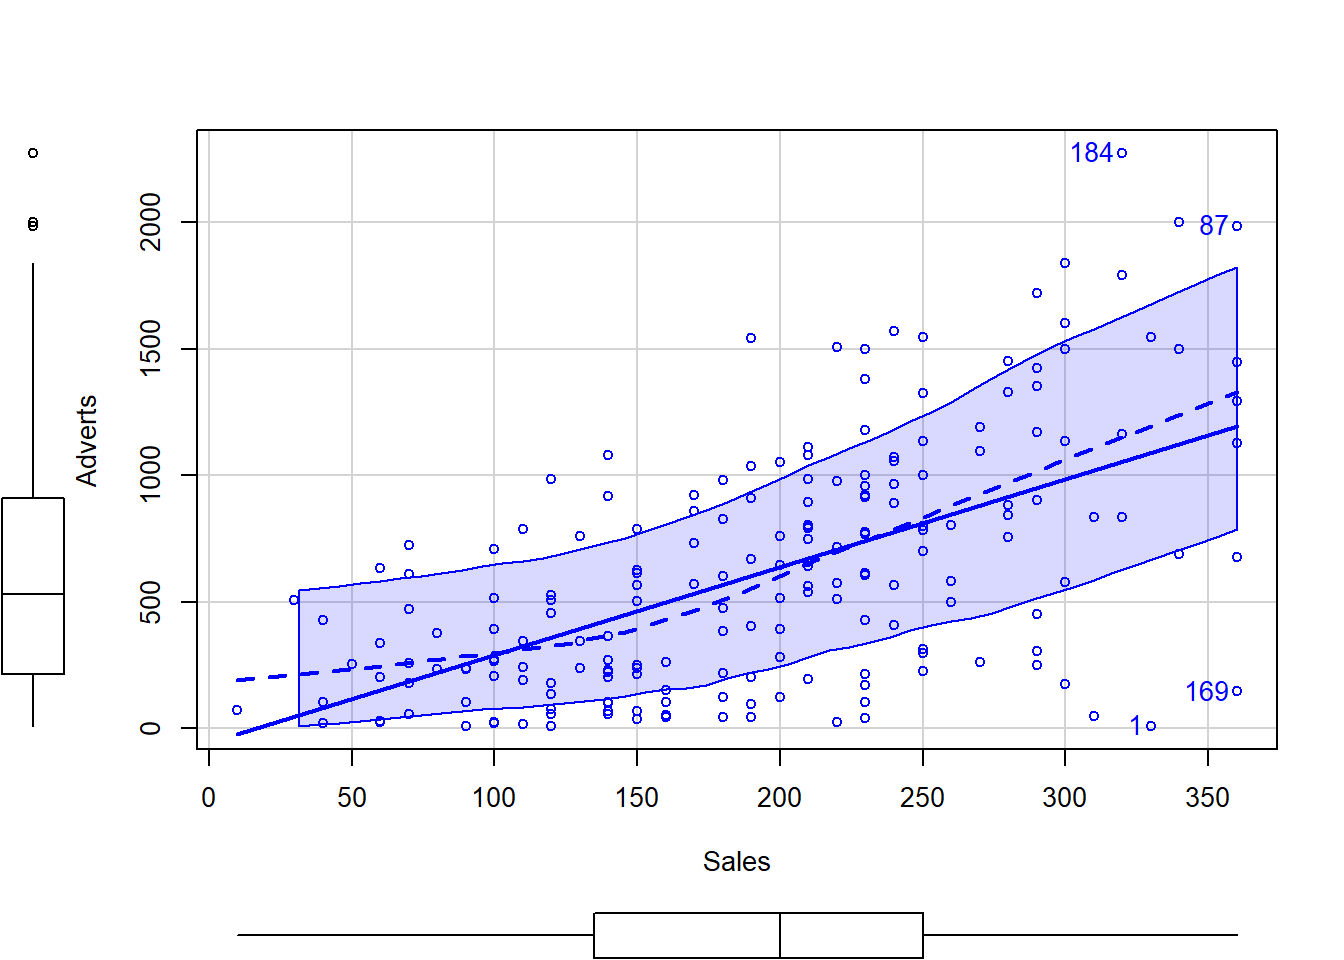
\includegraphics{Regresjon_Teori_files/figure-latex/unnamed-chunk-47-1.pdf}

Det som i den nederste av grafene over kalles ``hat values'' er et
vanlig mål for å finne observasjoner/caser som er relativt langt fra
senter av prediksjonsrommet og som derfor potensielt har stor
innflytelse på OLS-regresjonskoeffisientene (``leverage'') (Fox and
Weisberg 2019).

I den øverste grafen vises Cook's distance - et mål på vektet kvadratsum
for forskjellene mellom de individuelle elementene til koeffisienten.
Sagt på en annen måte: Vi bruker Cook's distance til å se hvilke
observasjoner/caser som kan påvirke modellen vår uforholdsmessig mye.
Dersom vi har mange caser med høy verdi på Cook's distance kan det være
en indikasjon på at lineær regresjon kanskje ikke er en egnet analyse
for det foreliggende datasettet.

Så hva er høy verdi på Cook's distance? Kilder som Cook and Weisberg
(1982) og Tabachnik and Fidell (2007) angir at verdier over 1 er
bekymringsfullt. Andre, som Fox (2020), advarer mot en ren numerisk
vurdering (og fremhever viktigheten av både grafisk presentasjon og
vurdering av hvert enkelt tilfelle).

La oss hente opp Cook's distance for de største verdiene for de enkelte
observasjoner:

\begin{verbatim}
##       1     169      42      55      10     125 
## 0.05716 0.05088 0.04055 0.02399 0.02374 0.02275
\end{verbatim}

Her kjenner vi igjen observasjonene 1, 169 og 42 som de med høyest verdi
på Cook's distance. Men vi ser også at verdien er relativt lave hvis man
tar utgangspunkt i 1 som bekymringsfullt, og trolig ikke noe vi ville
brydd oss mye om. For å vise eventuell justering av modellen som følge
av uteliggere viser vi likevel framgangsmåte.

Vi bør også undersøke ``added variable plots'' - i en regresjon kan
observasjonene ha både en individuell og en sammensatt/felles
påvirkning.

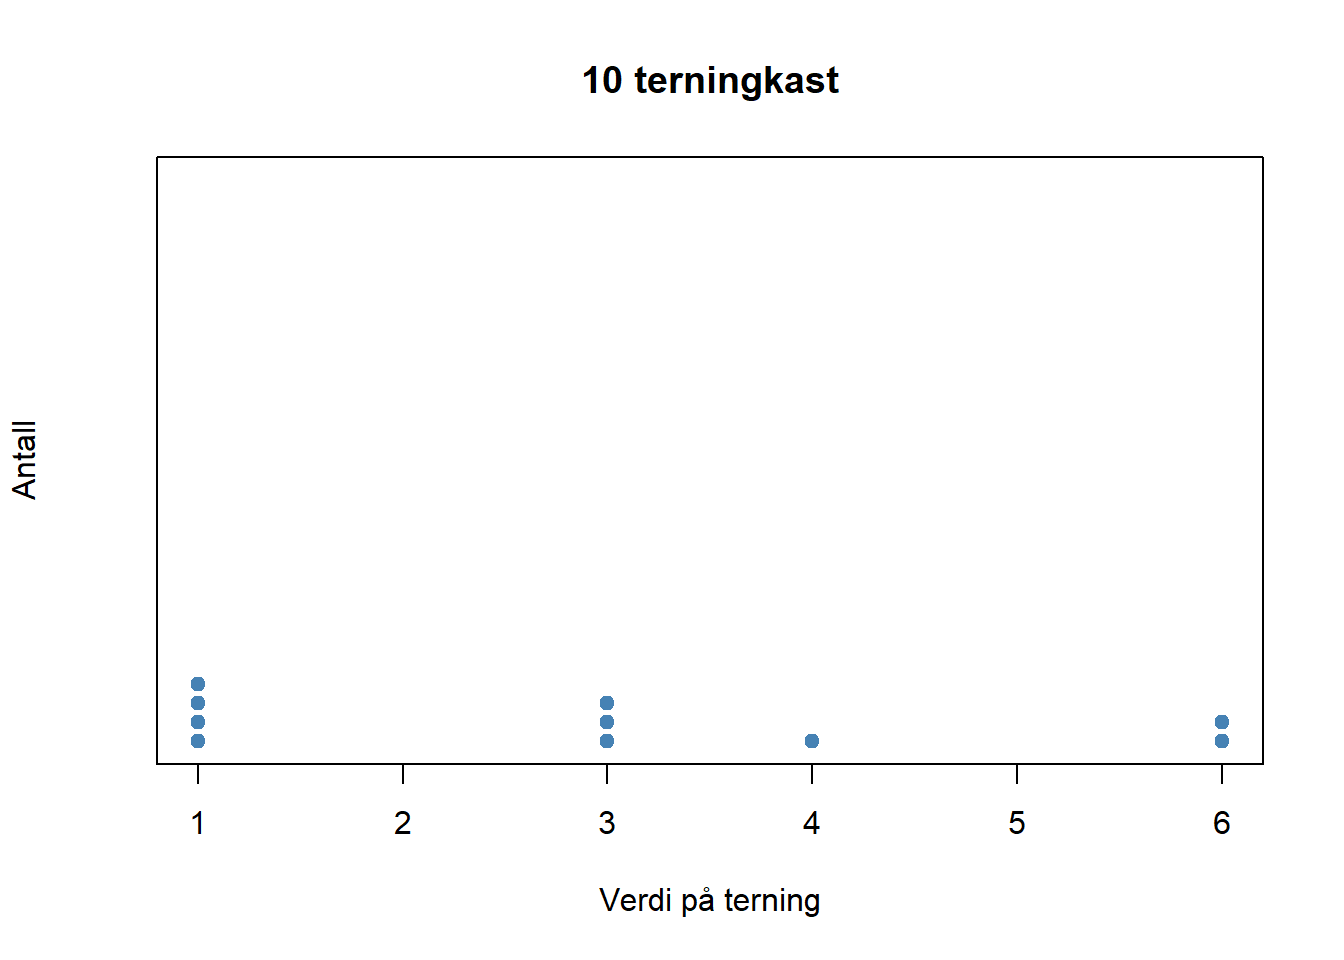
\includegraphics{Regresjon_Teori_files/figure-latex/unnamed-chunk-49-1.pdf}

Her sier Fox and Weisberg (2019), s.44 at ``Points at the extreme left
or right of the plot correspond to cases that have high leverage on the
corresponding coefficients and consequenlty are potentially
influential''.

Vi bør vurdere punktene over og vurdere om vi ønsker å lage en revidert
modell der vi tar ut veldig innflytelsesrike caser/observasjoner. Som
tidligere nevnt har vi ikke svært store verdier her, men la oss som et
eksempel si at vi ønsker å se om en modell uten observasjon 169. Vi
anbefaler å ta bort en og en observasjon siden (som nevnt)
observasjonene/casene har både en individuell og felles påvirkning.

\begin{verbatim}
## Calls:
## 1: lm(formula = Sales ~ Adverts, data = Field_OLS)
## 2: lm(formula = Sales ~ Adverts, data = Field_OLS, subset = -169)
## 
##             Model 1 Model 2
## (Intercept)  134.14  131.76
## SE             7.54    7.39
##                            
## Adverts     0.09612 0.09826
## SE          0.00963 0.00942
## 
\end{verbatim}

Som forventet ser vi ikke de store forskjellene. Vi kan ta bort de andre
observasjonene for illustrasjonens skyld:

\begin{verbatim}
## Calls:
## 1: lm(formula = Sales ~ Adverts, data = Field_OLS)
## 2: lm(formula = Sales ~ Adverts, data = Field_OLS, subset = -169)
## 3: lm(formula = Sales ~ Adverts, data = Field_OLS, subset = -c(1, 42, 169, 
##   184))
## 
##             Model 1 Model 2 Model 3
## (Intercept)  134.14  131.76  126.14
## SE             7.54    7.39    7.28
##                                    
## Adverts     0.09612 0.09826 0.10461
## SE          0.00963 0.00942 0.00942
## 
\end{verbatim}

Igjen, ikke de store endringene. Vi kan se at Intercept (\(\beta\)) går
litt ned etter hvert som vi tar bort caser, og betydningen av Adverts
går litt opp (men det er marginalt).

La oss, for eksempelets skyld, manipulere datasettet slik at en analyse
av Cook's distance ser slik ut:

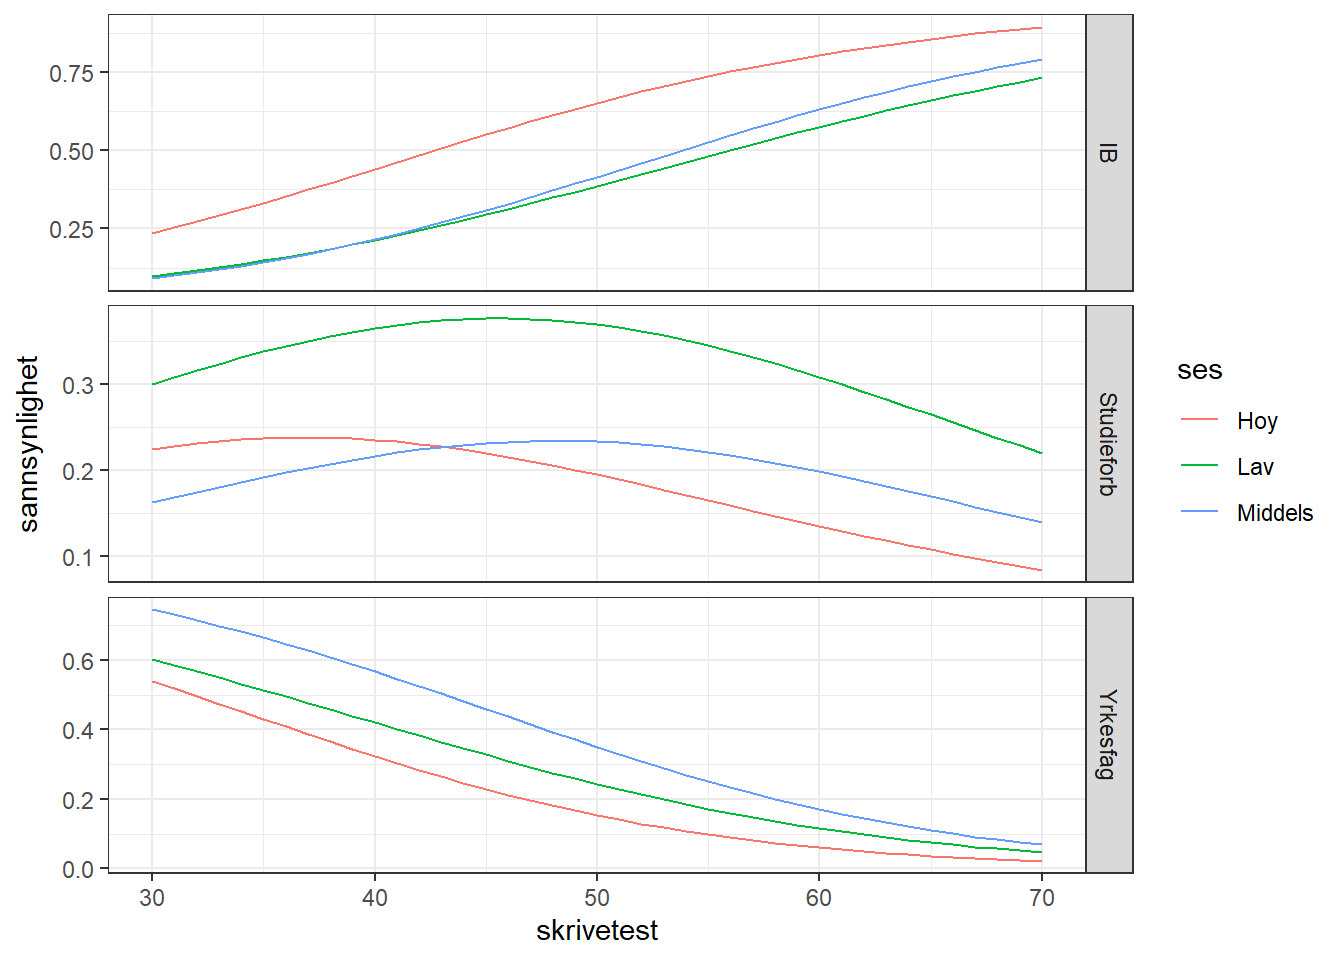
\includegraphics{Regresjon_Teori_files/figure-latex/unnamed-chunk-52-1.pdf}

Hvis vi nå kjører denne modellen opp mot en modell der vi tar bort 11 og
23 får vi:

\begin{verbatim}
## Calls:
## 1: lm(formula = Sales ~ Adverts, data = Field_datasett_OLS2)
## 2: lm(formula = Sales ~ Adverts, data = Field_datasett_OLS2, subset = -c(11,
##    23))
## 
##             Model 1 Model 2
## (Intercept)  183.77  134.14
## SE             5.97    7.64
##                            
## Adverts     0.01207 0.09621
## SE          0.00298 0.00999
## 
\end{verbatim}

Her ser vi koeffisienten for Adverts stiger fra 0.01 til 0.09, eller en
endring på 11.1\%.

\hypertarget{eventuell-analyse-av-revidert-modell}{%
\subsection{Eventuell analyse av revidert
modell}\label{eventuell-analyse-av-revidert-modell}}

Her vil vi prinsippet bare gjenta samme analyser som ved analyse av den
opprinnelige modellen.

\hypertarget{konklusjon-oppsummering-rapportering-av-resultater}{%
\subsection{Konklusjon / oppsummering / rapportering av
resultater}\label{konklusjon-oppsummering-rapportering-av-resultater}}

Vi viser her rapportering av en enkel lineær regresjonsanalyse etter
APA-standard:

En enkel lineær regresjon ble gjennomført for å predikere salgstall per
uke basert på sum brukt på reklame uka før lansering. Vi fant en
signifikant regresjonslikning (F(1,198) = 99.59, \(\beta\) = 134.14p
\textless{} .001) med en \(R^2\) på .335, 95\% CI {[}119.28, 149.00{]}.

\hypertarget{multippel-regresjonsanalyse}{%
\section{Multippel
regresjonsanalyse}\label{multippel-regresjonsanalyse}}

Vi skal gå gjennom et eksempel på multippel regresjonsanalyse, ved å
følge stegene under:

\begin{enumerate}
\def\labelenumi{\arabic{enumi}.}
\item
  Analyse av dataene
\item
  Evtentuelt valg av prediktorer ut fra analyse av dataene
\item
  Lage modell (kjøre regresjonsanalysen)
\item
  Analyse av resultatene (diagnostikk)
\item
  Sjekk av forutsetningene
\item
  Eventuell revisjon av modellen
\item
  Eventuell analyse av revidert modell
\item
  Konklusjon / oppsummering / rapportering av resultater
\end{enumerate}

\hypertarget{analyse-av-dataene}{%
\subsection{Analyse av dataene}\label{analyse-av-dataene}}

\hypertarget{referanser}{%
\section*{Referanser}\label{referanser}}
\addcontentsline{toc}{section}{Referanser}

\hypertarget{refs}{}
\begin{CSLReferences}{1}{0}
\leavevmode\vadjust pre{\hypertarget{ref-andersonTestGoodnessFit1954}{}}%
Anderson, T. W., and D. A. Darling. 1954. {``A {Test} of {Goodness} of
{Fit}.''} \emph{Journal of the American Statistical Association} 49
(268): 765--65. \url{https://doi.org/10.2307/2281537}.

\leavevmode\vadjust pre{\hypertarget{ref-andersonAsymptoticTheoryCertain1952b}{}}%
Anderson, Theodore W., and Donald A. Darling. 1952. {``Asymptotic Theory
of Certain "Goodness of Fit" Criteria Based on Stochastic Processes.''}
\emph{The Annals of Mathematical Statistics} 23 (2): 193--212.

\leavevmode\vadjust pre{\hypertarget{ref-berryUnderstandingRegressionAssumptions1993}{}}%
Berry, William D. 1993. \emph{Understanding Regression Assumptions}.
{Newbury Park, CA}: {Sage Publications}.

\leavevmode\vadjust pre{\hypertarget{ref-cookResidualsInfluenceRegression1982}{}}%
Cook, R. Dennis, and Sanford Weisberg. 1982. \emph{Residuals and
{Influence} in {Regression}}. {New York}: {Chapman and Hall}.

\leavevmode\vadjust pre{\hypertarget{ref-cummingIntroductionNewStatistics2017}{}}%
Cumming, Geoff, and Robert Calin-Jageman. 2017. \emph{Introduction to
the New Statistics: {Estimation}, Open Science, \& Beyond}. {New York}:
{Routledge}.

\leavevmode\vadjust pre{\hypertarget{ref-eikemoKvantitativAnalyseMed2007}{}}%
Eikemo, Terje Andreas, and Tommy Høyvarde Clausen, eds. 2007.
\emph{Kvantitativ Analyse Med {SPSS}. {En} Praktisk Innføring i
Kvantitative Analyseteknikker.} {Trondheim}: {Tapir Akademisk Forlag}.

\leavevmode\vadjust pre{\hypertarget{ref-fieldDiscoveringStatisticsUsing2009}{}}%
Field, Andy. 2009. \emph{Discovering {Statistics Using SPSS}}. Third.
{London}: {SAGE Publications Ltd}.

\leavevmode\vadjust pre{\hypertarget{ref-fieldDiscoveringStatisticsUsing2012}{}}%
Field, Andy, Jeremy Miles, and Zoë Field. 2012. \emph{Discovering
{Statistics Using R}}. {London}: {SAGE Publications}.

\leavevmode\vadjust pre{\hypertarget{ref-foxRegressionDiagnosticsIntroduction2020}{}}%
Fox, John. 2020. \emph{Regression {Diagnostics}: {An Introduction}.}
Second. {Los Angeles}: {Sage}.

\leavevmode\vadjust pre{\hypertarget{ref-foxCompanionAppliedRegression2019}{}}%
Fox, John, and Sanford Weisberg. 2019. \emph{An {R Companion} to
{Applied Regression}}. Third. {Thousand Oaks}: {SAGE}.

\leavevmode\vadjust pre{\hypertarget{ref-galarnykUnderstandingBoxplots2018}{}}%
Galarnyk, Michael. 2018. {``Understanding {Boxplots}.''} \emph{Towards
Data Science}.

\leavevmode\vadjust pre{\hypertarget{ref-greenHowManySubjects1991}{}}%
Green, Samuel B. 1991. {``How {Many Subjects Does It Take To Do A
Regression Analysis}.''} \emph{Multivariate Behavioral Research} 26 (3):
499--510. \url{https://doi.org/10.1207/s15327906mbr2603_7}.

\leavevmode\vadjust pre{\hypertarget{ref-hairjr.MultivariateDataAnalysis2010}{}}%
Hair Jr., Joseph H., William C. Black, Barry J. Babin, and Rolph E.
Anderson. 2010. \emph{Multivariate {Data Analysis}: {A Global
Perspective}}. Seventh. {Upper Saddle River, NJ}: {Pearson}.

\leavevmode\vadjust pre{\hypertarget{ref-harrisPrimerMultivariateStatistics2013}{}}%
Harris, Richard J. 2013. \emph{A {Primer} of {Multivariate Statistics}}.
Third. {New York}: {Psychology Press}.

\leavevmode\vadjust pre{\hypertarget{ref-hartmannELearningProjectSOGA2018}{}}%
Hartmann, K., J. Krois, and B. Waske. 2018. {``E-{Learning Project
SOGA}: {Statistics} and {Geospatial Data Analysis}.''}

\leavevmode\vadjust pre{\hypertarget{ref-hinkleAppliedStatisticsBehavioral2003}{}}%
Hinkle, Dennis E, William Wiersma, and Stephen G Jurs. 2003.
\emph{Applied Statistics for the Behavioral Sciences}. Fifth. {Belmont,
CA}: {Wadsworth, Cengagae Learning}.

\leavevmode\vadjust pre{\hypertarget{ref-kristensenAvhengigeMalefeilObservasjonsstudier2005}{}}%
Kristensen, Petter. 2005. {``Avhengige Målefeil i
Observasjonsstudier.''} \emph{Tidsskr Nor Lægeforen} 125: 173175--75.

\leavevmode\vadjust pre{\hypertarget{ref-lomaxStatisticalConceptsSecond2012}{}}%
Lomax, Richard G., and Debbie L. Hahs-Vaughn. 2012. \emph{Statistical
{Concepts}. {A Second Course}.} Fourth. {New York}: {Routledge}.

\leavevmode\vadjust pre{\hypertarget{ref-lovasStatistikkUniversiteterOg2013}{}}%
Løvås, Gunnar G. 2013. \emph{Statistikk for Universiteter Og Høgskoler}.
Third. {Oslo}: {Universitetsforlaget}.

\leavevmode\vadjust pre{\hypertarget{ref-macmahonBloodPressureStroke1990}{}}%
MacMahon, S, R Peto, R Collins, J Godwin, S MacMahon, J Cutler, P
Sorlie, et al. 1990. {``Blood Pressure, Stroke, and Coronary Heart
Disease: {Part} 1, Prolonged Differences in Blood Pressure: Prospective
Observational Studies Corrected for the Regression Dilution Bias.''}
\emph{Originally Published as Volume 1, Issue 8692} 335 (8692): 765--74.
\url{https://doi.org/10.1016/0140-6736(90)90878-9}.

\leavevmode\vadjust pre{\hypertarget{ref-mehmetogluInnforingStatistiskeDataanalyser2020}{}}%
Mehmetoglu, Mehmet, and Matthias Mittner. 2020. \emph{Innføring i {R}
for Statistiske Dataanalyser}. {Oslo}: {Universitetsforlaget}.

\leavevmode\vadjust pre{\hypertarget{ref-milesApplyingRegressionCorrelation2001}{}}%
Miles, Jeremy, and Mark Shevlin. 2001. \emph{Applying {Regression} \&
{Correlation}: {A Guide} for {Students} and {Researchers}}. {London}:
{Sage}.

\leavevmode\vadjust pre{\hypertarget{ref-navarroLearningStatisticsJamovi2019a}{}}%
Navarro, D. J., and D. R: Foxcroft. 2019. \emph{Learning Statistics with
Jamovi: A Tutorial for Psychology Students and Other Beginners.} 0.70
ed. \url{https://doi.org/10.24384/hgc3-7p15}.

\leavevmode\vadjust pre{\hypertarget{ref-nunallyPsychometricTheory1978}{}}%
Nunally, J. 1978. \emph{Psychometric {Theory}}. Second. {New York}:
{McGraw-Hill}.

\leavevmode\vadjust pre{\hypertarget{ref-razaliPowerComparisonsShapiroWilk2011}{}}%
Razali, Nornadiah Mohd, and Yap Bee Wah. 2011. {``Power Comparisons of
{Shapiro-Wilk}, {Kolmogorov-Smirnov}, {Lilliefors} and
{Anderson-Darling} Tests.''} \emph{Journal of Statistical Modeling and
Analytics} 2 (1): 21--33.

\leavevmode\vadjust pre{\hypertarget{ref-ringdalEnhetOgMangfold2007}{}}%
Ringdal, Kristen. 2007. \emph{Enhet Og Mangfold: Samfunnsvitenskapelig
Forskning Og Kvantitativ Metode}. {Bergen}: {Fagbokforl.}

\leavevmode\vadjust pre{\hypertarget{ref-schmidtRelativeEfficiencyRegression1971}{}}%
Schmidt, Frank L. 1971. {``The {Relative Efficiency} of {Regression} and
{Simple Unit Predictor Weights} in {Applied Differential Psychology}.''}
\emph{Educational and Psychological Measurement} 31 (3): 699--714.
\url{https://doi.org/10.1177/001316447103100310}.

\leavevmode\vadjust pre{\hypertarget{ref-stevensAppliedMultivariateStatistics1996}{}}%
Stevens, J. P. 1996. \emph{Applied Multivariate Statistics for the
Social Sciences}. Third. {Mahwah, NJ}: {Lawrence Erlbaum}.

\leavevmode\vadjust pre{\hypertarget{ref-tabachnikUsingMultivariateStatistics2007}{}}%
Tabachnik, B G, and L S Fidell. 2007. \emph{Using Multivariate
Statistics}. Fifth. {Boston}: {Pearson Education}.

\leavevmode\vadjust pre{\hypertarget{ref-thoresenMalefeilRegresjonsanalyse2003}{}}%
Thoresen, Magne. 2003. {``Målefeil i Regresjonsanalyse.''} \emph{Norsk
Epidemiologi} 13 (2): 257--63.

\leavevmode\vadjust pre{\hypertarget{ref-thraneAppliedRegressionAnalysis2019}{}}%
Thrane, Christer. 2019. \emph{Applied {Regression Analysis}. {Doing},
{Interpreting} and {Reporting}}. {London}: {Routledge}.

\leavevmode\vadjust pre{\hypertarget{ref-tukeyExploratoryDataAnalysis1977}{}}%
Tukey, John Wilder. 1977. \emph{Exploratory {Data Analysis}}. {Reading,
MA}: {Addison-Wesley}.

\leavevmode\vadjust pre{\hypertarget{ref-uboeStatistikkOkonomifag2014}{}}%
Ubøe, Jan. 2014. \emph{Statistikk for Økonomifag}. Fourth. {Oslo}:
{Gyldendal Akademisk}.

\end{CSLReferences}

\end{document}
